% Options for packages loaded elsewhere
\PassOptionsToPackage{unicode}{hyperref}
\PassOptionsToPackage{hyphens}{url}
%
\documentclass[
  english,
  man,floatsintext]{apa6}
\usepackage{amsmath,amssymb}
\usepackage{lmodern}
\usepackage{ifxetex,ifluatex}
\ifnum 0\ifxetex 1\fi\ifluatex 1\fi=0 % if pdftex
  \usepackage[T1]{fontenc}
  \usepackage[utf8]{inputenc}
  \usepackage{textcomp} % provide euro and other symbols
\else % if luatex or xetex
  \usepackage{unicode-math}
  \defaultfontfeatures{Scale=MatchLowercase}
  \defaultfontfeatures[\rmfamily]{Ligatures=TeX,Scale=1}
\fi
% Use upquote if available, for straight quotes in verbatim environments
\IfFileExists{upquote.sty}{\usepackage{upquote}}{}
\IfFileExists{microtype.sty}{% use microtype if available
  \usepackage[]{microtype}
  \UseMicrotypeSet[protrusion]{basicmath} % disable protrusion for tt fonts
}{}
\makeatletter
\@ifundefined{KOMAClassName}{% if non-KOMA class
  \IfFileExists{parskip.sty}{%
    \usepackage{parskip}
  }{% else
    \setlength{\parindent}{0pt}
    \setlength{\parskip}{6pt plus 2pt minus 1pt}}
}{% if KOMA class
  \KOMAoptions{parskip=half}}
\makeatother
\usepackage{xcolor}
\IfFileExists{xurl.sty}{\usepackage{xurl}}{} % add URL line breaks if available
\IfFileExists{bookmark.sty}{\usepackage{bookmark}}{\usepackage{hyperref}}
\hypersetup{
  pdftitle={Estimating individual subjective values of emotion regulation strategies},
  pdfauthor={Christoph Scheffel,1, Josephine Zerna,1, Anne Gärtner1, Denise Dörfel1, \& Alexander Strobel1},
  pdflang={en-EN},
  pdfkeywords={emotion regulation, regulatory effort, effort discounting, registered report, specification curve analysis},
  hidelinks,
  pdfcreator={LaTeX via pandoc}}
\urlstyle{same} % disable monospaced font for URLs
\usepackage{graphicx}
\makeatletter
\def\maxwidth{\ifdim\Gin@nat@width>\linewidth\linewidth\else\Gin@nat@width\fi}
\def\maxheight{\ifdim\Gin@nat@height>\textheight\textheight\else\Gin@nat@height\fi}
\makeatother
% Scale images if necessary, so that they will not overflow the page
% margins by default, and it is still possible to overwrite the defaults
% using explicit options in \includegraphics[width, height, ...]{}
\setkeys{Gin}{width=\maxwidth,height=\maxheight,keepaspectratio}
% Set default figure placement to htbp
\makeatletter
\def\fps@figure{htbp}
\makeatother
\setlength{\emergencystretch}{3em} % prevent overfull lines
\providecommand{\tightlist}{%
  \setlength{\itemsep}{0pt}\setlength{\parskip}{0pt}}
\setcounter{secnumdepth}{-\maxdimen} % remove section numbering
% Make \paragraph and \subparagraph free-standing
\ifx\paragraph\undefined\else
  \let\oldparagraph\paragraph
  \renewcommand{\paragraph}[1]{\oldparagraph{#1}\mbox{}}
\fi
\ifx\subparagraph\undefined\else
  \let\oldsubparagraph\subparagraph
  \renewcommand{\subparagraph}[1]{\oldsubparagraph{#1}\mbox{}}
\fi
% Manuscript styling
\usepackage{upgreek}
\captionsetup{font=singlespacing,justification=justified}

% Table formatting
\usepackage{longtable}
\usepackage{lscape}
% \usepackage[counterclockwise]{rotating}   % Landscape page setup for large tables
\usepackage{multirow}		% Table styling
\usepackage{tabularx}		% Control Column width
\usepackage[flushleft]{threeparttable}	% Allows for three part tables with a specified notes section
\usepackage{threeparttablex}            % Lets threeparttable work with longtable

% Create new environments so endfloat can handle them
% \newenvironment{ltable}
%   {\begin{landscape}\centering\begin{threeparttable}}
%   {\end{threeparttable}\end{landscape}}
\newenvironment{lltable}{\begin{landscape}\centering\begin{ThreePartTable}}{\end{ThreePartTable}\end{landscape}}

% Enables adjusting longtable caption width to table width
% Solution found at http://golatex.de/longtable-mit-caption-so-breit-wie-die-tabelle-t15767.html
\makeatletter
\newcommand\LastLTentrywidth{1em}
\newlength\longtablewidth
\setlength{\longtablewidth}{1in}
\newcommand{\getlongtablewidth}{\begingroup \ifcsname LT@\roman{LT@tables}\endcsname \global\longtablewidth=0pt \renewcommand{\LT@entry}[2]{\global\advance\longtablewidth by ##2\relax\gdef\LastLTentrywidth{##2}}\@nameuse{LT@\roman{LT@tables}} \fi \endgroup}

% \setlength{\parindent}{0.5in}
% \setlength{\parskip}{0pt plus 0pt minus 0pt}

% \usepackage{etoolbox}
\makeatletter
\patchcmd{\HyOrg@maketitle}
  {\section{\normalfont\normalsize\abstractname}}
  {\section*{\normalfont\normalsize\abstractname}}
  {}{\typeout{Failed to patch abstract.}}
\patchcmd{\HyOrg@maketitle}
  {\section{\protect\normalfont{\@title}}}
  {\section*{\protect\normalfont{\@title}}}
  {}{\typeout{Failed to patch title.}}
\makeatother
\shorttitle{Subjective values of emotion regulation strategies}
\keywords{emotion regulation, regulatory effort, effort discounting, registered report, specification curve analysis\newline\indent Word count: X}
\usepackage{lineno}

\linenumbers
\usepackage{csquotes}
\usepackage{booktabs}
\usepackage{longtable}
\usepackage{array}
\usepackage{multirow}
\usepackage{wrapfig}
\usepackage{float}
\usepackage{colortbl}
\usepackage{pdflscape}
\usepackage{tabu}
\usepackage{threeparttable}
\usepackage{threeparttablex}
\usepackage[normalem]{ulem}
\usepackage{makecell}
\usepackage{xcolor}
\usepackage{setspace}\doublespacing
\usepackage[final]{pdfpages}
\usepackage{chngcntr}
\ifxetex
  % Load polyglossia as late as possible: uses bidi with RTL langages (e.g. Hebrew, Arabic)
  \usepackage{polyglossia}
  \setmainlanguage[]{english}
\else
  \usepackage[main=english]{babel}
% get rid of language-specific shorthands (see #6817):
\let\LanguageShortHands\languageshorthands
\def\languageshorthands#1{}
\fi
\ifluatex
  \usepackage{selnolig}  % disable illegal ligatures
\fi
\newlength{\cslhangindent}
\setlength{\cslhangindent}{1.5em}
\newlength{\csllabelwidth}
\setlength{\csllabelwidth}{3em}
\newenvironment{CSLReferences}[2] % #1 hanging-ident, #2 entry spacing
 {% don't indent paragraphs
  \setlength{\parindent}{0pt}
  % turn on hanging indent if param 1 is 1
  \ifodd #1 \everypar{\setlength{\hangindent}{\cslhangindent}}\ignorespaces\fi
  % set entry spacing
  \ifnum #2 > 0
  \setlength{\parskip}{#2\baselineskip}
  \fi
 }%
 {}
\usepackage{calc}
\newcommand{\CSLBlock}[1]{#1\hfill\break}
\newcommand{\CSLLeftMargin}[1]{\parbox[t]{\csllabelwidth}{#1}}
\newcommand{\CSLRightInline}[1]{\parbox[t]{\linewidth - \csllabelwidth}{#1}\break}
\newcommand{\CSLIndent}[1]{\hspace{\cslhangindent}#1}

\title{Estimating individual subjective values of emotion regulation strategies}
\author{Christoph Scheffel\textsuperscript{$\dagger{}$,1}, Josephine Zerna\textsuperscript{$\dagger{}$,1}, Anne Gärtner\textsuperscript{1}, Denise Dörfel\textsuperscript{1}, \& Alexander Strobel\textsuperscript{1}}
\date{}


\authornote{

The authors made the following contributions. Christoph Scheffel: Conceptualization, Methodology, Funding acquisition, Formal analysis, Investigation, Project administration, Software, Visualization, Writing - original draft preparation, Writing - review \& editing; Josephine Zerna: Conceptualization, Methodology, Funding acquisition, Investigation, Project administration, Software, Writing - review \& editing; Anne Gärtner: Formal analysis, Writing - review \& editing; Denise Dörfel: Conceptuatlization, Writing - review \& editing; Alexander Strobel: Conceptualization, Writing - review \& editing. \textsuperscript{$\dagger{}$} Christoph Scheffel and Josephine Zerna contributed equally to this work.

Correspondence concerning this article should be addressed to Christoph Scheffel, Zellescher Weg 17, 01069 Dresden, Germany. E-mail: \href{mailto:christoph_scheffel@tu-dresden.de}{\nolinkurl{christoph\_scheffel@tu-dresden.de}}

}

\affiliation{\vspace{0.5cm}\textsuperscript{1} Faculty of Psychology, Technische Universität Dresden, 01069 Dresden, Germany}

\abstract{
Individuals have a repertoire of emotion regulation (ER) strategies at their disposal, which they can use more or less flexibly.
In ER flexibility research, strategies that facilitate goal achievement are considered adaptive and therefore are subjectively valuable.
Individuals are motivated to reduce their emotional arousal effectively and to avoid cognitive effort.
Perceived costs of ER strategies in the form of effort, however, are highly subjective.
Subjective values (SVs) should therefore represent a trade-off between effectiveness and subjectively required cognitive effort.
However, SVs of ER strategies have not been determined so far.
We present a paradigm that is suitable for determining individual SVs of ER strategies.
Using a multilevel modelling approach, it will be investigated whether individual SVs can be explained by effectiveness (subjective arousal, facial muscle activity) and subjective effort.
Relations of SVs to personality traits will be explored
}



\begin{document}
\maketitle

\renewcommand\thesection{\Alph{section}}
\counterwithout{figure}{section}
\setcounter{figure}{0}

\begin{center}\rule{0.5\linewidth}{0.5pt}\end{center}

\hypertarget{introduction}{%
\section{1. Introduction}\label{introduction}}

Every day we are confronted with stressful or emotionally demanding situations.
The ability to modify emotional experiences, expressions, and physiological reactions\textsuperscript{1} to regulate emotions is an important cognitive skill.
It is therefore not surprising that emotion regulation (ER) has substantial implications for well-being and adaptive functioning.\textsuperscript{2}
Different strategies can be used to regulate emotions, namely situation selection, situation modification, attentional deployment, cognitive change, and response modification,\textsuperscript{1} and, following the taxonomy of Powers and LaBar,\textsuperscript{3} individuals can implement ER strategies by means of different tactics.
So called antecedent-focused strategies, e.g., attentional deployment and cognitive change, take effect early in the emotion generation process.\textsuperscript{1}
In contrast, response modification takes place late in the process and is therefore conceptualized as a response-focused strategy.\textsuperscript{1}
This postulated temporal sequence of ER strategies influences their effectiveness.
It is meta-analytically proven that all mentioned strategies reduce subjective emotional arousal.\textsuperscript{4}
Distraction as a tactic of attentional deployment and (expressive) suppression as a tactic of response modulation showed small to medium effect sizes on measures of emotional experience (distraction: \emph{d\textsubscript{+}} = 0.27; suppression: \emph{d\textsubscript{+}} = 0.27).
Distancing as tactic of cognitive change showed the highest effectiveness with an effect size of \emph{d\textsubscript{+}} = 0.45.\textsuperscript{4}
Moreover it is known that ER strategies reduce physiological arousal, measured via EMG in the region of the \emph{corrugator supercilii}.\textsuperscript{5}
So these tactics from three different strategies proved to be effective in the short term.
However, in order to be able to make a statement on their general benefit, longer-term consequences must also be considered.
Especially strategies that do not put the emotional content of the situation into a neutral perspective (i.e., distraction and suppression) are presumed to be disadvantageous in the longer term.
Long-term consequences of subjectively reported habitual use of emotion regulation strategies for affect and well-being have been discussed.\textsuperscript{6}
Especially suppression is generally associated with poorer outcomes (i.e., more negative affect, lower general well-being), which led to the assumption of \emph{adaptive} and \emph{maladaptive} strategies.
For example, it could be shown that maladaptive ER strategies mediate the effect between neuroticism and depressive symptoms.\textsuperscript{7}
Also, a number of ER strategies is linked to psychological disorders (for meta-analytic review, see).\textsuperscript{8}

The postulation of \emph{adaptive} and \emph{maladaptive} strategies was put in a new perspective with the concept of ER flexibility.
Similar to other psychological domains, e.g., attention and goal pursuit, \emph{maladaptive} now refers to inflexible strategy use or use of strategies that are hindering the achievement of goals.\textsuperscript{9}
Adaptive flexible ER requires having a large repertoire of ER strategies.\textsuperscript{9}
For example, greater ER variability is related to reduced negative affect and therefore beneficial in daily life.\textsuperscript{10}
Strategies have to be chosen from the repertoire that are useful for goal achieving.
Evidence from other contexts (e.g., intertemporal choice,)\textsuperscript{11} shows that subjective values (SVs) are attributed to the choice options on the basis of which the decision is made.
Research on ER choice has identified numerous factors that influence the choice of ER strategies, which can be seen as indirect evidence for factors influencing SVs.
For example, it was shown that the intensity of a stimulus or situation plays a role in the choice.\textsuperscript{12}
Higher intensity of the stimulus leads to a choice of rather disengaging strategies, like distraction.\textsuperscript{12,13}
Further influencing factors are for example extrinsic motivation (e.g.~monetary incentives), motivational determinants (i.e.~hedonic regulatory goals), and effort.\textsuperscript{13,14}
Especially for effort, in our previous work we could show that the choice for an ER strategy is mainly influenced by effort.\textsuperscript{14}
In this study, participants used the strategies distancing and suppression while inspecting emotional pictures.
Afterwards they could choose, which strategy they want to use again.
Participants tended to re-apply the strategy that was less effortful, even though it was not the most effective one - in this case: Suppression.
Interestingly, the choice was independent of self reported habitual use of suppression and reappraisal.
What has been missing in research on ER choice so far is information regarding the strategy \emph{not} chosen.
People choose a strategy that they prefer, for different, relatively well-known reasons.
However, nothing is revealed about the strategy that is not chosen.

The postulation of \emph{adaptive} and \emph{maladaptive} strategies was put into a new perspective with the concept of ER flexibility.
Similar to other psychological domains such as attention and goal pursuit, \emph{maladaptive} now refers to inflexible strategy use or use of strategies that are hindering the achievement of goals.\textsuperscript{9}
In contrast, \emph{adaptive} ER requires having a large repertoire of ER strategies to choose from\textsuperscript{9} and choosing the strategy that is useful for goal achieving in a particular situation.
This greater ER variability has been shown to be related to reduced negative affect.\textsuperscript{10}
The process of choosing an ER strategy from one's own repertoire likely shares similarities with other contexts such as intertemporal choice, in which individuals assign subjective values to every choice option.\textsuperscript{11}
Additionally, there are ER-specific influences on choice behaviour such as the intensity of the stimulus or situation, which leads to a choice of rather disengaging strategies like distraction, extrinsic motivation (e.g.~monetary incentives), motivational determinants (i.e.~hedonic regulatory goals), and effort.\textsuperscript{13,14}
Effort in particular appeared to be the main factor in ER choice behaviour in our previous work.\textsuperscript{14}
In that study, participants used the strategies distancing and suppression while inspecting emotional pictures, and could choose which strategy they wanted to use again.
Participants tended to re-apply the strategy that was less effortful, even though it was not the most effective one for them - in this case: Suppression.
Interestingly, the choice was independent of self reported habitual use of suppression and reappraisal.
Research on ER choice has shown that individuals choose a strategy that they prefer for different, relatively well-known reasons.
However, nothing has been investigated regarding the strategy that is \emph{not} chosen.

We assume that people choose the strategy that has the highest value for them at that moment.
The value is determined against the background of goal achievement in the specific situation: A strategy is highly valued if it facilitates goal achievement.\textsuperscript{9}
One certainly central goal is the regulation of negative affect.
A second, intrinsic and rather less obvious goal is the avoidance of effort.\textsuperscript{15}
When given the choice, most individuals prefer tasks that are less effortful.\textsuperscript{16}
We assume that both aspects are set off against each other by individuals to determine individual subjective values (SVs) of ER strategies: A strategy is more valuable if it can reduce emotional arousal \emph{and} is less effortful.
SVs of ER Strategies could be helpful to describe the ER repertoire\textsuperscript{9} more comprehensively.
Depending on the flexibility of a person, different patterns of SVs could be conceivable: A person with high flexibility would show relatively high SVs for a number of strategies.
This would mean that all strategies are a good option for goal achievement.
A second person with less flexibilty, however, would show high SVs only for one strategy, or for no strategy at all.
This in turn would mean that no strategy is a good choice to achieve goals.

However, so far we have not seen any attempt in ER choice research to determine individual SVs of ER strategies.
To investigate this question, the individual subjective values of each strategy available for selection would have to be determined.
Promising approaches can be found in studies on difficulty levels of effortful cognitive tasks.\\
Individual SVs of effortful cognitive tasks have been quantified using the Cognitive Effort Discounting Paradigm (COG-ED).\textsuperscript{17}

\hypertarget{er-strategy-discounting}{%
\subsection{1.1 ER strategy discounting}\label{er-strategy-discounting}}

In the original study by Westbrook et al.,\textsuperscript{17} cognitive load was varied using the \emph{n}-back task, a working memory task that requires fast and accurate responses to sequentially presented stimuli.
Participants had to decide whether they wanted to repeat a higher \emph{n}-back level for a larger, fixed monetary reward, or a lower level for a smaller, varying reward.
In the current study, we want to use this paradigm to determine SVs of ER strategies.
In doing so, we need to make an important change: We have to adapt the assumption that the easiest \emph{n}-back level has the highest SV.
As we have shown in previous studies, there are large inter-individual differences in the preference and perceived subjective effort of ER strategies.\textsuperscript{14}
Moreover, there is nothing like an objectively easiest ER strategy.
Therefore, we have to add an additional step, which preceeds the other steps and where the option with the higher subjective value is determined.
In this step, the same monetary value (i.e., 1 EUR) is assigned to both options.
The assumption is that participants now choose the option that has the higher SV for them.
In the next step we return to the original paradigm.
The higher monetary value (i.e., 2 EUR) is assigned to the option that was not chosen in the first step and therefore is assumed to have the lower SV.
In the following steps, the lower value is changed in every iteration according to Westbrook et al.\textsuperscript{17} until the indifference point is reached.
This procedure will be repeated until all strategies have been compared.
The SV of each strategy is calculated as the mean of this strategy's SV from all comparisons.
In case a participant has a clear preference for one strategy, the SV of this strategy will be 1.
But our paradigm can also account for the case that a person does not have a clear preference.
Then no SV will be 1, but still, the SVs of all strategies can be interpreted as absolute values and in relation to the other strategy's SVs (see figure 1).
Additionally, we will test our adapted paradigm in a \emph{n}-back task and explore whether this paradigm can describe individuals that do not prefer the easiest \emph{n}-back option (see Zerna et al., \ldots).

\begin{figure}
\includegraphics[width=0.98\linewidth]{C:/Users/scheffel/Scheffel/Forschung/A_Projects/2021_CERED/CERED/99_Thinktank/Other/Paradigm_Scheme_T2} \caption{Exemplary visualisation of two response patterns. In the top half, the person has a clear preference for one of the three strategies. In the lower half, they have no clear preference and therefore show an inconsistent response pattern. This pattern can also be represented by our paradigm.}\label{fig:fig1}
\end{figure}

\hypertarget{the-present-study}{%
\subsection{1.2 The present study}\label{the-present-study}}

The aim of the present study is to evaluate if this paradigm is suitable for determining SVs of ER strategies.
As a manipulation check, we want to explore whether ER strategies distraction, distancing, and suppression effectively reduce emotional arousal and require cognitive effort. The following hypotheses are proposed for this purpose:

\begin{itemize}
\tightlist
\item
  H1a) Subjective arousal (arousal ratings) is lower after using an ER strategy (distraction, distancing, suppression) compared to active viewing.
\item
  H1b) Physiological arousal (EMG \emph{corrugator} activity) is lower after using an ER strategy (distraction, distancing, suppression) compared to active viewing.
\item
  H1c) Physiological arousal (EMG \emph{levator} activity) is lower after using an ER strategy (distraction, distancing, suppression) compared to active viewing.
\item
  H2a) Subjective effort (effort ratings) is greater after using an Er strategy (distraction, distancing, suppression) compared to active viewing.
\item
  H2b) The majority of participants ruse the strategy that was least effortful for them.
\end{itemize}

Further we want to explore which variables predict individual subjective values of ER strategies and whether effort is the best predictor for SVs of ER strategies with the following hypotheses:

\begin{itemize}
\tightlist
\item
  H3a) Subjective effort ratings negatively predict SVs of ER strategies.
\item
  H3b) Subjective arousal ratings negatively predict SVs of ER strategies.
\item
  H3c) EMG \emph{corrugator} activity negatively predict SVs of ER strategies.
\item
  H3d) EMG \emph{levator} activity negatively predict SVs of ER strategies.
\item
  H4a) SVs decline with increasing effort, even after controlling for task performance measured by subjective arousal ratings, \emph{corrugator} and \emph{levator} activity.
\end{itemize}

We also want to explore whether SVs are related to flexible emotion regulation:

\begin{itemize}
\tightlist
\item
  H5a) The higher the SV, the more likely the respective strategy is chosen.
\item
  H5b) SVs are lower and decline stronger when ER flexibility is lower.
\end{itemize}

Exploratorily, we want to investigate whether individual SVs are related to personality traits and how individual SVs of ER strategies relate to SVs of other tasks with different demand levels, namely \emph{n}-back.

\hypertarget{method}{%
\section{2. Method}\label{method}}

The R Markdown file used to analyze the data and write this document, as well as the raw data and the materials are freely available at github.com/ChScheffel/COG-ER-ED.
According to the 21-word-solution, ``we report how we determined our sample size, all data exclusions (if any), all manipulations, and all measures in the study'' in compliance with the 21-word-solution of open science.\textsuperscript{18}
A complete list of all measures assessed in the study will be found at the OSF (\url{https://osf.io/vnj8x/}) and GitHub (github.com/ChScheffel/COG-ER-ED).
All procedures performed in this study were in accordance with the ethical standards of the institutional and/or national research committee and with the 1964 Helsinki declaration and its later amendments or comparable ethical standards.

\hypertarget{ethics-information}{%
\subsection{2.1 Ethics information}\label{ethics-information}}

\hypertarget{pilot-data}{%
\subsection{2.2 Pilot data}\label{pilot-data}}

The procedure described above was tested in a pilot study with \(N=16\) participants (9 female; age: \(M = 24.10\text{ }\pm\text{ }SD = 3.60\)).
Results showed significant higher subjective (\ldots{} and physiological ?!) arousal for active viewing of negative pictures, compared to active viewing of neutral pictures.
However, ER strategies could not reduce subjective arousal compared to active viewing of negative pictures.
Yet we found accordance with our previous studies\textsuperscript{14} that the use of ER strategies compared to active viewing was associated with increased subjective effort.

\hypertarget{design}{%
\subsection{2.3 Design}\label{design}}

Young, healthy participants (aged 18 to 30 years) will be recruited using the software \emph{ORSEE}\textsuperscript{19} at the Technische Universität Dresden.
Participants will be invited to fill out an online survey containing different questionnaires to assess broad and narrow personality traits and measures of well-being.
The study consists of two lab sessions, which take place in a shielded cabin with constant lighting.
Before each session, participants receive information about the respective experimental procedure and provide informed consent.
At the beginning of the first session participants fill out a demographic questionnaire and complete an n-Back task with the levels one to four.
Then, they complete an ED procedure on screen, followed by a random repetition of one n-back level.
The second session, containing the ER paradigm, takes place exactly one week after session one.
Participants provide informed consent and receive written instructions on the ER paradigm and ER strategies that they should apply.
A brief training ensures that all participants are able to implement the ER strategies.
Next, electrodes to measure EMG are being attached and the ER paradigm is conducted.
Participants receive 30.00€ or course credit as compensation.
Study data are being collected and managed using REDCap electronic data capture tools hosted at Technische Universität Dresden.\textsuperscript{20,21}

\hypertarget{psychometric-measures}{%
\subsubsection{2.3.1 Psychometric measures}\label{psychometric-measures}}

The online survey contains a number of questionnaires: General psychological well-being is assessed using the German version of the WHO-5 scale.\textsuperscript{22,23}
To capture the construct of resilience, the German version 10-item-form of the Connor-Davidson resilience Scale (CD-RISC)\textsuperscript{26} is used.
Dispositional use of ER is assessed using the German version of the Emotion Regulation Questionnaire (ERQ).\textsuperscript{6,27}
For the assessment of ER ability we use the Flexible Emotion Regulation Scale (FlexER).\textsuperscript{28}
Implicit theories of willpower in emotion control are assessed using the implicit theories questionnaire from.\textsuperscript{29}
To assess Need for Cognition, the German version short form of the Need for Cognition Scale\textsuperscript{30,31} is used.
To assess self-control, sum scores of the German versions of the following questionnaires are used:\textsuperscript{32} the Self-Regulation Scale (SRS),\textsuperscript{33} the Brief Self-Control Scale (BSCS);\textsuperscript{34}{]},\textsuperscript{35} and the Barratt Impulsiveness Scale (BIS-11).\textsuperscript{36,37}
Attentional control is assessed using the Attentional Control Scale (ACS).\textsuperscript{38}

\hypertarget{emotion-regulation-paradigm}{%
\subsubsection{2.3.2 Emotion regulation paradigm}\label{emotion-regulation-paradigm}}

The ER paradigm roughly consists of three parts that will be described in the following.

\emph{Part one: ER task.} Part one is a standard ER task in a block design (see Figure X), similar to paradigms previously used by our group.\textsuperscript{14}
Participants are told to actively view neutral and negative pictures (see \protect\hyperlink{ux5cux23stimuli}{2.3.3}) or to regulate all upcoming emotions by means of distraction, distancing, and expressive suppression, respectively.
Every participant first has the condition ``active viewing-neutral'' that serves as a baseline condition.
During this block, 20 neutral pictures are presented.
Participants are asked to ``actively view all pictures and permit all emotions that may arise.'' In the second block, participants actively viewe negative pictures.
During the third, fourth, and fifth block, participants see negative pictures and are asked to regulate their emotions using distraction, distancing, and suppression.
In order to achieve distraction, participants are asked to think of a geometric object or an everyday activity, like brushing their teeth.
During distancing, participants are asked to ``take the position of a non-involved observer, thinking about the picture in a neutral way.'' Participants are told not to re-interpret the situation or attaching a different meaning to the situation.
During suppression, participants are told to ``suppress their emotional facial expression.'' They should imagine being observed by a third person that should not be able to tell just by looking at the facial expression whether the person is looking at an emotional picture.
Participants are instructed not to suppress their thoughts or change their facial expression to the opposite.\textsuperscript{14}
All participants receive written instruction and complete a training session.
After the training session, participants are asked about their applied ER strategies to avoid misapplication.
The order of the three regulation blocks (distraction, distancing, and suppression) is randomized between participants.

\emph{Part two: ER effort discounting.} In the second part, ER effort discounting takes place.
The procedure of the discounting follows the COG-ED paradigm by Westbrook et al.\textsuperscript{17} with major change.
We use the following adaption that allows the computation of SVs for different strategies without presuming that all individuals would inherently evaluate the same strategy as the easiest one: For each possible pairing (distraction vs.~distancing, distraction vs.~suppression, and distancing vs.~suppression), two strategies with monetary values are presented.
The order of the comparisons is randomized.
Because there is no strategy that is objectively more difficult, we added an initial comparison that begins with the option ``1 EUR for strategy A or 1 EUR for strategy B''.
The strategy that is not chosen is assigned the value of 2 EUR.
From this point on, comparisons between strategies follow the original COG-ED paradigm.\textsuperscript{17}
Participants are instructed to decide as realistically as possible, imagining the displayed money would really be up for election.

\emph{Part three: ER choice.} After the discounting part, participants choose which of the three ER strategies (distraction, distancing or suppression) they want to re-apply.
Importantly, there are no further instruction on what basis they should make their decision.
Participants should make their decision freely, according to the criteria they consider important for themselves.
However, participants are asked to state the reasons for the decision afterwards.
As soon as they have decided, they see the respective instruction and the block with another 20 negative pictures starts.

\hypertarget{stimuli}{%
\subsubsection{2.3.3 Stimuli}\label{stimuli}}

Pictures used in the paradigm were selected from the Emotional Picture Set (EmoPicS)\textsuperscript{39} and the International Affective Picture System (IAPS).\textsuperscript{40}
The 20 neutral pictures (Valence (V): \emph{M} \(\pm\) \emph{SD} = 4.81 \(\pm\) 0.51; Arousal (A): \emph{M} \(\pm\) \emph{SD} = 3 \(\pm\) 0.65) depicted content related to the categories persons, objects, and scenes.
Further, 100 negative pictures, featuring categories animals, body, disaster, disgust, injury, suffering, violence, and weapons, were used.
An evolutionary algorithm\textsuperscript{41} was used to cluster these pictures into five sets with comparable valence and arousal values (set one: V: \emph{M} \(\pm\) \emph{SD} = 2.84 \(\pm\) 0.57, A: \emph{M} \(\pm\) \emph{SD} = 5.62 \(\pm\) 0.34; set two: V: \emph{M} \(\pm\) \emph{SD} = 2.64 \(\pm\) 0.46, A: \emph{M} \(\pm\) \emph{SD} = 5.58 \(\pm\) 0.35; set three: V: \emph{M} \(\pm\) \emph{SD} = 2.82 \(\pm\) 0.62, A: \emph{M} \(\pm\) \emph{SD} = 5.60 \(\pm\) 0.39; set four: V: \emph{M} \(\pm\) \emph{SD} = 2.65 \(\pm\) 0.75, A: \emph{M} \(\pm\) \emph{SD} = 5.61 \(\pm\) 0.41; set five: V: \emph{M} \(\pm\) \emph{SD} = 2.74 \(\pm\) 0.70, A: \emph{M} \(\pm\) \emph{SD} = 5.63 \(\pm\) 0.37).
A complete list of all pictures and their classification into sets can be found in supplementary material X.

\hypertarget{electromyography}{%
\subsubsection{2.3.4 Electromyography}\label{electromyography}}

Two bipolar electromyograph (EMG) measures will be recorded in the region of the \emph{corrugator supercilii} and the \emph{levator labii} using Brain Vision Recorder (Brain Products Inc., Gilching, Germany).
Passive surface Ag/AgCl electrodes (0.7 mm diameter, 10 mm distance between electrodes) filled with electrolyte gel will be used.
Data will be sampled at 1000 Hz.
To measure \emph{corrugator EMG}, electrodes will be applied to the abraded and cleaned skin on the left \emph{corrugator supercilii}, and to measure \emph{levator EMG}, electrodes were applied in the region of the \emph{levator labii}.
The ground electrode will be placed at the left \emph{Mastoid}.
A 20 Hz high pass (order 8), a 300 Hz low pass (order 8), and a 50 Hz notch filter will be applied to both signals.
Afterwards, the signals will be rectified and segmented.
EMG data will be baseline-corrected to -200 ms to 0 ms to stimulus onset.
Last, the sampling rate is changed to 100 Hz and the AUC for the interval of 6000 ms stimulus presentation extracted for every stimulus.

\hypertarget{sampling-plan}{%
\subsection{2.4 Sampling plan}\label{sampling-plan}}

Participants will be healthy adults in the age of 18 to 30, recruited using the software \emph{ORSEE}\textsuperscript{19} at the Technische Universität Dresden.
Participants will be excluded from participation if they do not fluently speak German, have current or a history of psychological disorders or neurological trauma, or report to take medication.
Sample size calculation is done using \emph{G*Power}.\textsuperscript{42,43}
In a meta-analysis of Zaehringer and colleagues,\textsuperscript{5} effect sizes of ER on peripheral-physiological measures were reported.
To find an effect of \(d=-0.32\) of ER on \emph{corrugator} muscle activity with \(\alpha=.05\) and \(\beta=.95\), data of least \(N=85\) have to be analyzed.
Power analyses of all other hypotheses yielded smaller sample sizes.
However, if participants withdraw from study participation, technical failures occur, or experimenter considers the participant for not suitable for study participation (e.g., because the participant does not follow instructions or shows great fatigue), respective data will also be excluded from further analyses.
Therefore, we aim to collect data of 90 participants.

\hypertarget{analysis-plan}{%
\subsection{2.5 Analysis plan}\label{analysis-plan}}

All statistical analyses will be performed using \emph{RStudio} (version 1.4.1717)\textsuperscript{44}and \emph{R} (version 4.1.0)\textsuperscript{45} for Windows.
The level of significance was set to \(\alpha=.05\).

\emph{Effects of emotion regulation on arousal and effort} To examine impact of valence of emotional pictures on subjective arousal, an repeated measures analysis of variance (rmANOVA) with the factor valence (neutral and negative) for strategy active viewing will be conducted for behavioral data (subjective arousal ratings).
To investigate the effect of the tree ER strategies on subjective arousal, another rmANOVA was conducted with the factor strategy (active viewing, distraction, distancing, and suppression) for subjective arousal ratings of negative pictures.
To examine the impact of valence on the emotional facial reaction, an rmANOVA with the factor valence (neutral and negative) for strategy active viewing was conducted for EMG activity of \emph{corrugator} and \emph{levator}.
A further rmANOVA with the factor strategy (active viewing, distraction, distancing, and suppression) was conducted for EMG activity to examine the effects of ER strategies on the emotional facial reaction.
To examine the effect of ER strategies on cognitive effort, an rmANOVA with the factor strategy (active viewing, distraction, distancing, and suppression) for subjective effort ratings was conducted.
Greenhouse-Geisser-corrected \(p\)-values and degrees of freedom were reported when assumption of sphericity was violated.
Proportion of explained variance \(\eta_{p}^{2}\) was reported as a measure of effect size.
If indicated by the data, estimated marginal means will be computed as post-hoc contrasts.

\emph{Subjective values of emotion regulation strategies} For each ER strategy, SVs were calculated as follows: first, the value 0.015625 was added to or subtracted from the last monetary value of the flexible strategy, depending on the participant's last choice.
Second, the resulting (monetary) value will be divided by 2.00 €.
The final SV for each participant will be computed by averaging all final SVs of each strategy.
The resulting values will be entered in a rmANOVA to compare the SVs of the three strategies (distraction, distancing, and suppression) to explore for group effects.
Again, estimated, marginal means will be computed as post-hoc contrasts.

To investigate, whether individual SVs predict ER choice, a Chi-squared test with predicted choice (highest SV of each participant) and actual choice will be computed.
Furthermore, an ordinal logistic regression with dependent variable choice and independent variables SVs of each strategy will be computed.

To explore the association between subjective arousal, physiological arousal, and subjective effort on SVs, a multilevel model (MLM) will be specified using the \(lmerTest\) package.\textsuperscript{46}
First, ER strategies will be re-coded and centered for each subject according to their individual SVs: The strategy with the highest SV will be coded as -1, the strategy with the second highest SV 0, and the strategy with the lowest SV will be coded as 1.
Restricted maximum likelihood (REML) will be applied to fit the model.
A random slopes model of SVs including subjective effort (effort ratings), subjective arousal (arousal ratings), and physiological arousal (\emph{corrugator} activity and \emph{levator} activity) as level-1-predictor will be specified.
\[
SV \sim strategy\ + \text{effort rating} + \text{arousal rating} + corrugator \text{ activity} + levator \text{ activity} + (strategy|subject)
\] Level-1-predictors will be centered within cluster.\textsuperscript{47}
Residuals of the final model will be inspected visually.
Intraclass correlation coefficient (ICC), \(\rho\), will be reported for each model (null model, as well as full model).

The influence of personality traits on SVs will be investigated exploratorily.
Therefore, the MLM specified above will be extended by the level-2-predictors NFC and self-control.

The association between flexible ER and SVs of ER strategies will be investigated with a regression using the \(intercept\) and \(slope\) of each participants' SVs to predict threir FlexER score.
Therefore, SVs will be ordered by magnitude firstly.
Secondly, for each participant a linear model will be built to estimate the individual \(intercept\) and \(slope\).

For each result of the analyses both, \(p\)-values and Bayes factor \(BF10\), calculated using the \emph{BayesFactor} package,\textsuperscript{48} will be reported.

\hypertarget{data-availability}{%
\subsection{Data availability}\label{data-availability}}

The data of this study can be downloaded from \href{https://osf.io/vnj8x/}{osf.io/vnj8x/}.

\hypertarget{code-availability}{%
\subsection{Code availability}\label{code-availability}}

The paradigm code, as well as the R Markdown file used to analyze the data and write this document is available at our \href{https://github.com/ChScheffel/CERED}{Github repository}.

\hypertarget{references}{%
\section{References}\label{references}}

\begingroup
\setlength{\parindent}{-0.5in}
\setlength{\leftskip}{0.5in}

\hypertarget{refs}{}
\begin{CSLReferences}{0}{0}
\leavevmode\hypertarget{ref-Gross1998antecedent}{}%
\CSLLeftMargin{1. }
\CSLRightInline{Gross, J. J. Antecedent- and response-focused emotion regulation: Divergent consequences for experience, expression, and physiology. \emph{Journal of Personality and Social Psychology} \textbf{74}, 224--37 (1998).}

\leavevmode\hypertarget{ref-Gross1998emerging}{}%
\CSLLeftMargin{2. }
\CSLRightInline{Gross, J. J. The emerging field of emotion regulation: An integrative review. \emph{Review of General Psychology} \textbf{2}, 271--299 (1998).}

\leavevmode\hypertarget{ref-Powers2019}{}%
\CSLLeftMargin{3. }
\CSLRightInline{Powers, J. P. \& LaBar, K. S. Regulating emotion through distancing: A taxonomy, neurocognitive model, and supporting meta-analysis. \emph{Neuroscience and Biobehavioral Reviews} \textbf{96}, 155--173 (2019).}

\leavevmode\hypertarget{ref-Webb2012}{}%
\CSLLeftMargin{4. }
\CSLRightInline{Webb, T. L., Miles, E. \& Sheeran, P. Dealing with feeling: A meta-analysis of the effectiveness of strategies derived from the process model of emotion regulation. \emph{Psychological Bulletin} \textbf{138}, 775--808 (2012).}

\leavevmode\hypertarget{ref-Zaehringer2020}{}%
\CSLLeftMargin{5. }
\CSLRightInline{Zaehringer, J., Jennen-Steinmetz, C., Schmahl, C., Ende, G. \& Paret, C. Psychophysiological effects of downregulating negative emotions: Insights from a meta-analysis of healthy adults. \emph{Front Psychol} \textbf{11}, 470 (2020).}

\leavevmode\hypertarget{ref-GrossJohn2003}{}%
\CSLLeftMargin{6. }
\CSLRightInline{Gross, J. J. \& John, O. P. Individual differences in two emotion regulation processes: Implications for affect, relationships, and well-being. \emph{Journal of Personality and Social Psychology} \textbf{85}, 348--62 (2003).}

\leavevmode\hypertarget{ref-Yoon2013}{}%
\CSLLeftMargin{7. }
\CSLRightInline{Yoon, K. L., Maltby, J. \& Joormann, J. A pathway from neuroticism to depression: Examining the role of emotion regulation. \emph{Anxiety, Stress, \& Coping} \textbf{26}, 558--72 (2013).}

\leavevmode\hypertarget{ref-Aldao2010}{}%
\CSLLeftMargin{8. }
\CSLRightInline{Aldao, A., Nolen-Hoeksema, S. \& Schweizer, S. Emotion-regulation strategies across psychopathology: A meta-analytic review. \emph{Clinical Psychology Review} \textbf{30}, 217--237 (2010).}

\leavevmode\hypertarget{ref-Aldao2015}{}%
\CSLLeftMargin{9. }
\CSLRightInline{Aldao, A., Sheppes, G. \& Gross, J. J. Emotion regulation flexibility. \emph{Cognitive Therapy and Research} \textbf{39}, 263--278 (2015).}

\leavevmode\hypertarget{ref-Blanke2020}{}%
\CSLLeftMargin{10. }
\CSLRightInline{Blanke, E. S. \emph{et al.} Mix it to fix it: Emotion regulation variability in daily life. \emph{Emotion} \textbf{20}, 473--485 (2020).}

\leavevmode\hypertarget{ref-Kable2007}{}%
\CSLLeftMargin{11. }
\CSLRightInline{Kable, J. W. \& Glimcher, P. W. The neural correlates of subjective value during intertemporal choice. \emph{Nat Neurosci} \textbf{10}, 1625--33 (2007).}

\leavevmode\hypertarget{ref-Sheppes2011}{}%
\CSLLeftMargin{12. }
\CSLRightInline{Sheppes, G., Scheibe, S., Suri, G. \& Gross, J. J. Emotion-regulation choice. \emph{Psychological Science} \textbf{22}, 1391--6 (2011).}

\leavevmode\hypertarget{ref-Sheppes2014}{}%
\CSLLeftMargin{13. }
\CSLRightInline{Sheppes, G. \emph{et al.} Emotion regulation choice: A conceptual framework and supporting evidence. \emph{Journal of Experimental Psychology: General} \textbf{143}, 163--81 (2014).}

\leavevmode\hypertarget{ref-Scheffel2021}{}%
\CSLLeftMargin{14. }
\CSLRightInline{Scheffel, C. \emph{et al.} Effort beats effectiveness in emotion regulation choice: Differences between suppression and distancing in subjective and physiological measures. \emph{Psychophysiology} \textbf{00}, e13908 (2021).}

\leavevmode\hypertarget{ref-Inzlicht2018}{}%
\CSLLeftMargin{15. }
\CSLRightInline{Inzlicht, M., Shenhav, A. \& Olivola, C. Y. The effort paradox: Effort is both costly and valued. \emph{Trends Cogn Sci} \textbf{22}, 337--349 (2018).}

\leavevmode\hypertarget{ref-Hull1943}{}%
\CSLLeftMargin{16. }
\CSLRightInline{Hull, C. L. \emph{Principles of behavior: An introduction to behavior theory}. (Appleton-Century-Crofts, 1943).}

\leavevmode\hypertarget{ref-Westbrook2013}{}%
\CSLLeftMargin{17. }
\CSLRightInline{Westbrook, A., Kester, D. \& Braver, T. S. What is the subjective cost of cognitive effort? {Load}, trait, and aging effects revealed by economic preference. \emph{PLOS ONE} \textbf{8}, e68210 (2013).}

\leavevmode\hypertarget{ref-Simmons2012}{}%
\CSLLeftMargin{18. }
\CSLRightInline{Simmons, J. P., Nelson, L. D. \& Simonsohn, U. A. A 21 word solution. \emph{SSRN Electronic Journal} (2012) doi:\href{https://doi.org/10.2139/ssrn.2160588}{10.2139/ssrn.2160588}.}

\leavevmode\hypertarget{ref-Greiner2015}{}%
\CSLLeftMargin{19. }
\CSLRightInline{Greiner, B. Subject pool recruitment procedures: {Organizing} experiments with {ORSEE}. \emph{Journal of the Economic Science Association} \textbf{1}, 114--125 (2015).}

\leavevmode\hypertarget{ref-Harris2009}{}%
\CSLLeftMargin{20. }
\CSLRightInline{Harris, P. A. \emph{et al.} Research electronic data capture ({REDCap})---{A} metadata-driven methodology and workflow process for providing translational research informatics support. \emph{Journal of Biomedical Informatics} \textbf{42}, 377--381 (2009).}

\leavevmode\hypertarget{ref-Harris2019}{}%
\CSLLeftMargin{21. }
\CSLRightInline{Harris, P. A. \emph{et al.} The {REDCap} consortium: {Building} an international community of software platform partners. \emph{Journal of Biomedical Informatics} \textbf{95}, 103208 (2019).}

\leavevmode\hypertarget{ref-Bech2004}{}%
\CSLLeftMargin{22. }
\CSLRightInline{Bech, P. Measuring the dimensions of psychological general well-being by the WHO-5. \emph{Quality of life newsletter} \textbf{32}, 15--16 (2004).}

\leavevmode\hypertarget{ref-Braehler2007}{}%
\CSLLeftMargin{23. }
\CSLRightInline{Brähler, E., Mühlan, H., Albani, C. \& Schmidt, S. Teststatistische pr{ü}fung und normierung der deutschen versionen des EUROHIS-QOL lebensqualit{ä}t-index und des WHO-5 wohlbefindens-index. \emph{Diagnostica} \textbf{53}, 83--96 (2007).}

\leavevmode\hypertarget{ref-Connor2003}{}%
\CSLLeftMargin{24. }
\CSLRightInline{Connor, K. M. \& Davidson, J. R. Development of a new resilience scale: The connor-davidson resilience scale (CD-RISC). \emph{Depression and Anxiety} \textbf{18}, 76--82 (2003).}

\leavevmode\hypertarget{ref-Sarubin2015}{}%
\CSLLeftMargin{25. }
\CSLRightInline{Sarubin, N. \emph{et al.} First analysis of the 10-and 25-item german version of the connor-davidson resilience scale (CD-RISC) regarding psychometric properties and components. \emph{Zeitschrift Fur Gesundheitspsychologie} \textbf{23}, 112--122 (2015).}

\leavevmode\hypertarget{ref-Campbell-Sills2007}{}%
\CSLLeftMargin{26. }
\CSLRightInline{Campbell-Sills, L. \& Stein, M. B. Psychometric analysis and refinement of the connor-davidson resilience scale (CD-RISC): Validation of a 10-item measure of resilience. \emph{Journal of Traumatic Stress} \textbf{20}, 1019--28 (2007).}

\leavevmode\hypertarget{ref-Abler2009}{}%
\CSLLeftMargin{27. }
\CSLRightInline{Abler, B. \& Kessler, H. Emotion regulation questionnaire - a german version of the ERQ by gross and john. \emph{Diagnostica} \textbf{55}, 144--152 (2009).}

\leavevmode\hypertarget{ref-Doerfel2019}{}%
\CSLLeftMargin{28. }
\CSLRightInline{Dörfel, D., Gärtner, A. \& Strobel, A. A new self-report instrument for measuring emotion regulation flexibility. \emph{Society for Affective Science (SAS) Annual Conference} (2019).}

\leavevmode\hypertarget{ref-Bernecker2017}{}%
\CSLLeftMargin{29. }
\CSLRightInline{Bernecker, K. \& Job, V. Implicit theories about willpower in resisting temptations and emotion control. \emph{Zeitschrift Fur Psychologie-Journal of Psychology} \textbf{225}, 157--166 (2017).}

\leavevmode\hypertarget{ref-Cacioppo1982}{}%
\CSLLeftMargin{30. }
\CSLRightInline{Cacioppo, J. T. \& Petty, R. E. The need for cognition. \emph{Journal of Personality and Social Psychology} \textbf{42}, 116--131 (1982).}

\leavevmode\hypertarget{ref-Bless1994}{}%
\CSLLeftMargin{31. }
\CSLRightInline{Bless, H., Wanke, M., Bohner, G., Fellhauer, R. F. \& Schwarz, N. Need for cognition - a scale measuring engagement and happiness in cognitive tasks. \emph{Zeitschrift Für Sozialpsychologie} \textbf{25}, 147--154 (1994).}

\leavevmode\hypertarget{ref-Paschke2016}{}%
\CSLLeftMargin{32. }
\CSLRightInline{Paschke, L. M. \emph{et al.} Individual differences in self-reported self-control predict successful emotion regulation. \emph{Social Cognitive and Affective Neuroscience} \textbf{11}, 1193--204 (2016).}

\leavevmode\hypertarget{ref-Schwarzer1999}{}%
\CSLLeftMargin{33. }
\CSLRightInline{Schwarzer, R., Diehl, M. \& Schmitz, G. S. Self-regulation scale. (1999).}

\leavevmode\hypertarget{ref-Tangney2004}{}%
\CSLLeftMargin{34. }
\CSLRightInline{Tangney, J. P., Baumeister, R. F. \& Boone, A. L. High self-control predicts good adjustment, less pathology, better grades, and interpersonal success. \emph{Journal of Personality} \textbf{72}, 271--324 (2004).}

\leavevmode\hypertarget{ref-Sproesser2011}{}%
\CSLLeftMargin{35. }
\CSLRightInline{Sproesser, G., Strohbach, S., Schupp, H. \& Renner, B. Candy or apple? How self-control resources and motives impact dietary healthiness in women. \emph{Appetite} \textbf{56}, 784--787 (2011).}

\leavevmode\hypertarget{ref-Patton1995}{}%
\CSLLeftMargin{36. }
\CSLRightInline{Patton, J. H., Stanford, M. S. \& Barratt, E. S. Factor structure of the barratt impulsiveness scale. \emph{Journal of Clinical Psychology} \textbf{51}, 768--774 (1995).}

\leavevmode\hypertarget{ref-Hartmann2011}{}%
\CSLLeftMargin{37. }
\CSLRightInline{Hartmann, A. S., Rief, W. \& Hilbert, A. Psychometric properties of the german version of the barratt impulsiveness scale, version 11 (BIS-11) for adolescents. \emph{Perceptual and Motor Skills} \textbf{112}, 353--368 (2011).}

\leavevmode\hypertarget{ref-Derryberry2002}{}%
\CSLLeftMargin{38. }
\CSLRightInline{Derryberry, D. \& Reed, M. A. Anxiety-related attentional biases and their regulation by attentional control. \emph{Journal of abnormal psychology} \textbf{111}, 225--236 (2002).}

\leavevmode\hypertarget{ref-Wessa2010}{}%
\CSLLeftMargin{39. }
\CSLRightInline{Wessa, M. \emph{et al.} EmoPicS: Subjective und psychophysiologische evalueation neuen bildmaterials für die klinisch-biopsychologische forschung. \emph{Zeitschrift für Klinische Psychologie und Psychotherapie} \textbf{39}, 77 (2010).}

\leavevmode\hypertarget{ref-Lang2008}{}%
\CSLLeftMargin{40. }
\CSLRightInline{Lang, P. J., Bradley, M. M. \& Cuthbert, B. N. \emph{International affective picture system (IAPS): Affective ratings of pictures and instruction manual}. (University of Florida, 2008).}

\leavevmode\hypertarget{ref-Yu2010}{}%
\CSLLeftMargin{41. }
\CSLRightInline{Yu, X. \& Gen, M. \emph{Introduction to evolutionary algorithms}. (Springer Science \& Business Media, 2010).}

\leavevmode\hypertarget{ref-Faul2007}{}%
\CSLLeftMargin{42. }
\CSLRightInline{Faul, F., Erdfelder, E., Lang, A.-G. \& Buchner, A. G*{Power} 3: {A} flexible statistical power analysis program for the social, behavioral, and biomedical sciences. \emph{Behavior Research Methods} \textbf{39}, 175--191 (2007).}

\leavevmode\hypertarget{ref-Faul2009}{}%
\CSLLeftMargin{43. }
\CSLRightInline{Faul, F., Erdfelder, E., Buchner, A. \& Lang, A.-G. Statistical power analyses using {G}*{Power} 3.1: {Tests} for correlation and regression analyses. \emph{Behavior Research Methods} \textbf{41}, 1149--1160 (2009).}

\leavevmode\hypertarget{ref-RStudioTeam2020}{}%
\CSLLeftMargin{44. }
\CSLRightInline{RStudio Team. {RStudio}: {Integrated} development for {R}. (2020).}

\leavevmode\hypertarget{ref-RCore2021}{}%
\CSLLeftMargin{45. }
\CSLRightInline{R Core Team. \emph{R: A language and environment for statistical computing}. (R Foundation for Statistical Computing, 2021).}

\leavevmode\hypertarget{ref-Kuznetsova2017}{}%
\CSLLeftMargin{46. }
\CSLRightInline{Kuznetsova, A., Brockhoff, P. B. \& Christensen, R. H. B. {lmerTest} package: Tests in linear mixed effects models. \emph{Journal of Statistical Software} \textbf{82}, 1--26 (2017).}

\leavevmode\hypertarget{ref-Enders2007}{}%
\CSLLeftMargin{47. }
\CSLRightInline{Enders, C. K. \& Tofighi, D. Centering predictor variables in cross-sectional multilevel models: {A} new look at an old issue. \emph{Psychological Methods} \textbf{12}, 121--138 (2007).}

\leavevmode\hypertarget{ref-Morey2021}{}%
\CSLLeftMargin{48. }
\CSLRightInline{Morey, R. D. \& Rouder, J. N. \emph{{BayesFactor}: {Computation} of {Bayes} factors for common designs}. (2021).}

\end{CSLReferences}

\endgroup

\newpage

\hypertarget{acknowledgements}{%
\section{Acknowledgements}\label{acknowledgements}}

This research is partly funded by the German Research Foundation (DFG) as part of the Collaborative Research Center (CRC) 940.
Additionally, we have applied for funding of the participants' compensation from centralized funds of the Faculty of Psychology at Technische Universität Dresden.
Applications for the centralized funds will be reviewed in May.
Regardless of whether or not this additional funding will be granted, the study can commence immediately.
The funders have/had no role in study design, data collection and analysis, decision to publish or preparation of the manuscript.

\hypertarget{author-contributions}{%
\section{Author Contributions}\label{author-contributions}}

CS, AS, and JZ conceptualized the study and its methodology.
CS and JZ acquired funding, investigated, administered the project, and wrote the software.
CS, JZ, and AG did the formal analysis.
CS and JZ visualized the results, and prepared the original draft.
All authors reviewed, edited, and approved the final version of the manuscript.

\hypertarget{competing-interests}{%
\section{Competing Interests}\label{competing-interests}}

The authors declare no competing interests.

\newpage
\setcounter{figure}{0}

\hypertarget{figures-and-figure-captions}{%
\section{Figures and figure captions}\label{figures-and-figure-captions}}

\newpage
\begin{figure}
\includegraphics[width=0.98\linewidth]{C:/Users/scheffel/Scheffel/Forschung/A_Projects/2021_CERED/CERED/99_Thinktank/Other/Paradigm_Scheme_T2} \caption{ }\label{fig:fig1appendix}
\end{figure}

\emph{Figure 1.} Exemplary visualisation of two response patterns. In the top half, the person has a clear preference for one of the three strategies. In the lower half, they have no clear preference and therefore show an inconsistent response pattern. This pattern can also be represented by our paradigm.
\# Design Table

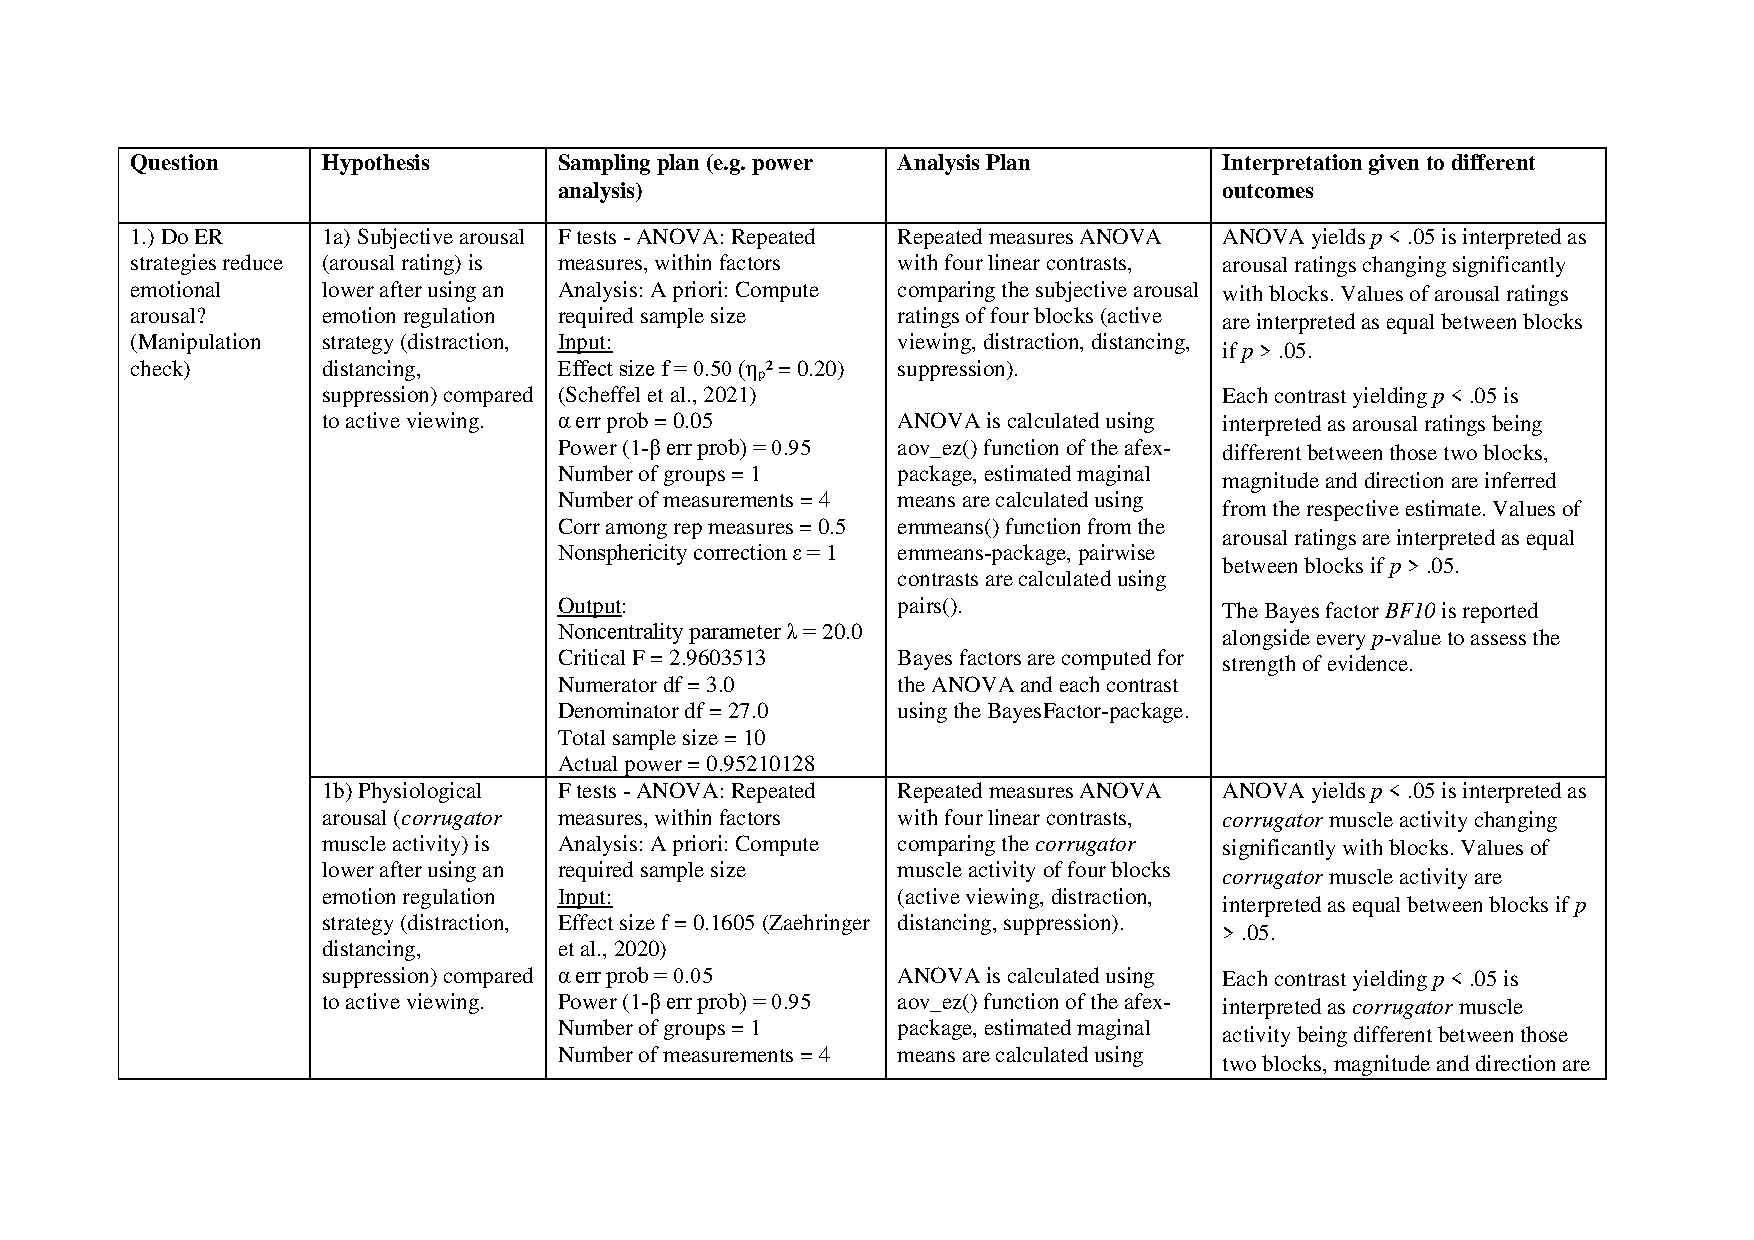
\includepdf[pages={-}, landscape=true]{Supplement/Design_Table_T2.pdf}

\newpage

\hypertarget{supplement}{%
\section{Supplement}\label{supplement}}

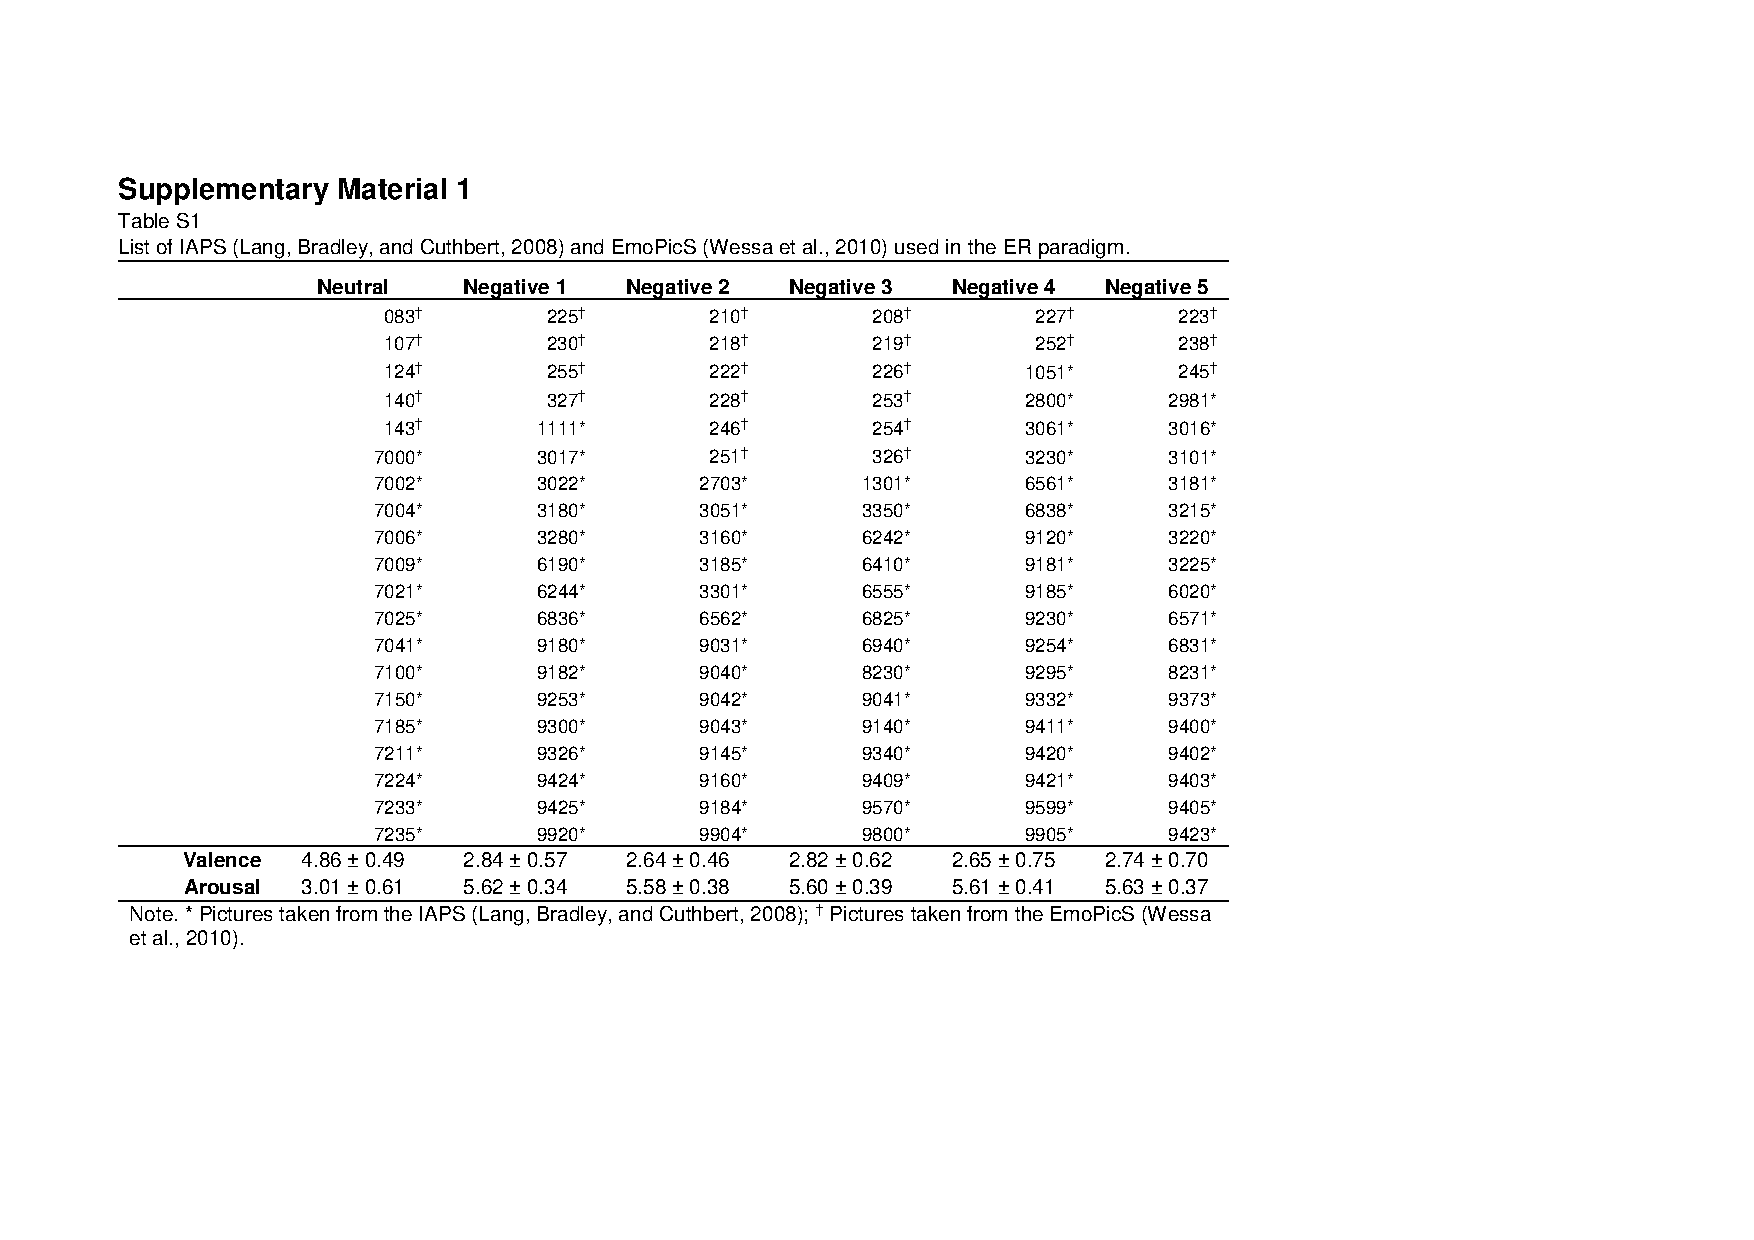
\includepdf[pages={-}, landscape=true]{Supplement/StimList_Suppl.pdf}

\newpage

\hypertarget{pilot-study-subjective-arousal-in-the-conditions-active-viewing---neutral-and-active-viewing---negative}{%
\subsection{Pilot study: Subjective arousal in the conditions ``Active viewing - neutral'' and ``Active viewing - negative''}\label{pilot-study-subjective-arousal-in-the-conditions-active-viewing---neutral-and-active-viewing---negative}}

ANOVA:

\begin{tabular}{l|l|l|l|l|l}
\hline
Effect & df & MSE & F & ges & p.value\\
\hline
block & 1, 15 & 3895.91 & 34.32 *** & .475 & <.001\\
\hline
\end{tabular}

\(BF10=\) 1,244.99

Paired contrasts:

\begin{table}[H]

\begin{center}
\begin{threeparttable}

\caption{\label{tab:unnamed-chunk-3}Paired contrasts for the rmANOVA comparing subjective arousal of negative and neutral pictures in the condition "active viewing".}

\begin{tabular}{lllllllll}
\toprule
Contrast & \multicolumn{1}{c}{Estimate} & \multicolumn{1}{c}{$SE$} & \multicolumn{1}{c}{$df$} & \multicolumn{1}{c}{$t$} & \multicolumn{1}{c}{$p$} & \multicolumn{1}{c}{$BF10$} & \multicolumn{1}{c}{$\eta_{p}^{2}$} & \multicolumn{1}{c}{$95\% CI$}\\
\midrule
$View_{neutral} - View_{negative}$ & -129.28 & 22.07 & 15.00 & -5.86 & 0.00 & 794.78 & 0.70 & {}[0.43, 1.00]\\
\bottomrule
\addlinespace
\end{tabular}

\begin{tablenotes}[para]
\normalsize{\textit{Note.} $SE$ = standard error, $df$ = degrees of freedom, $t$ = $t$-statistic, $p$ = $p$-value, CI = confidence interval.}
\end{tablenotes}

\end{threeparttable}
\end{center}

\end{table}

Figure:

\begin{figure}[H]
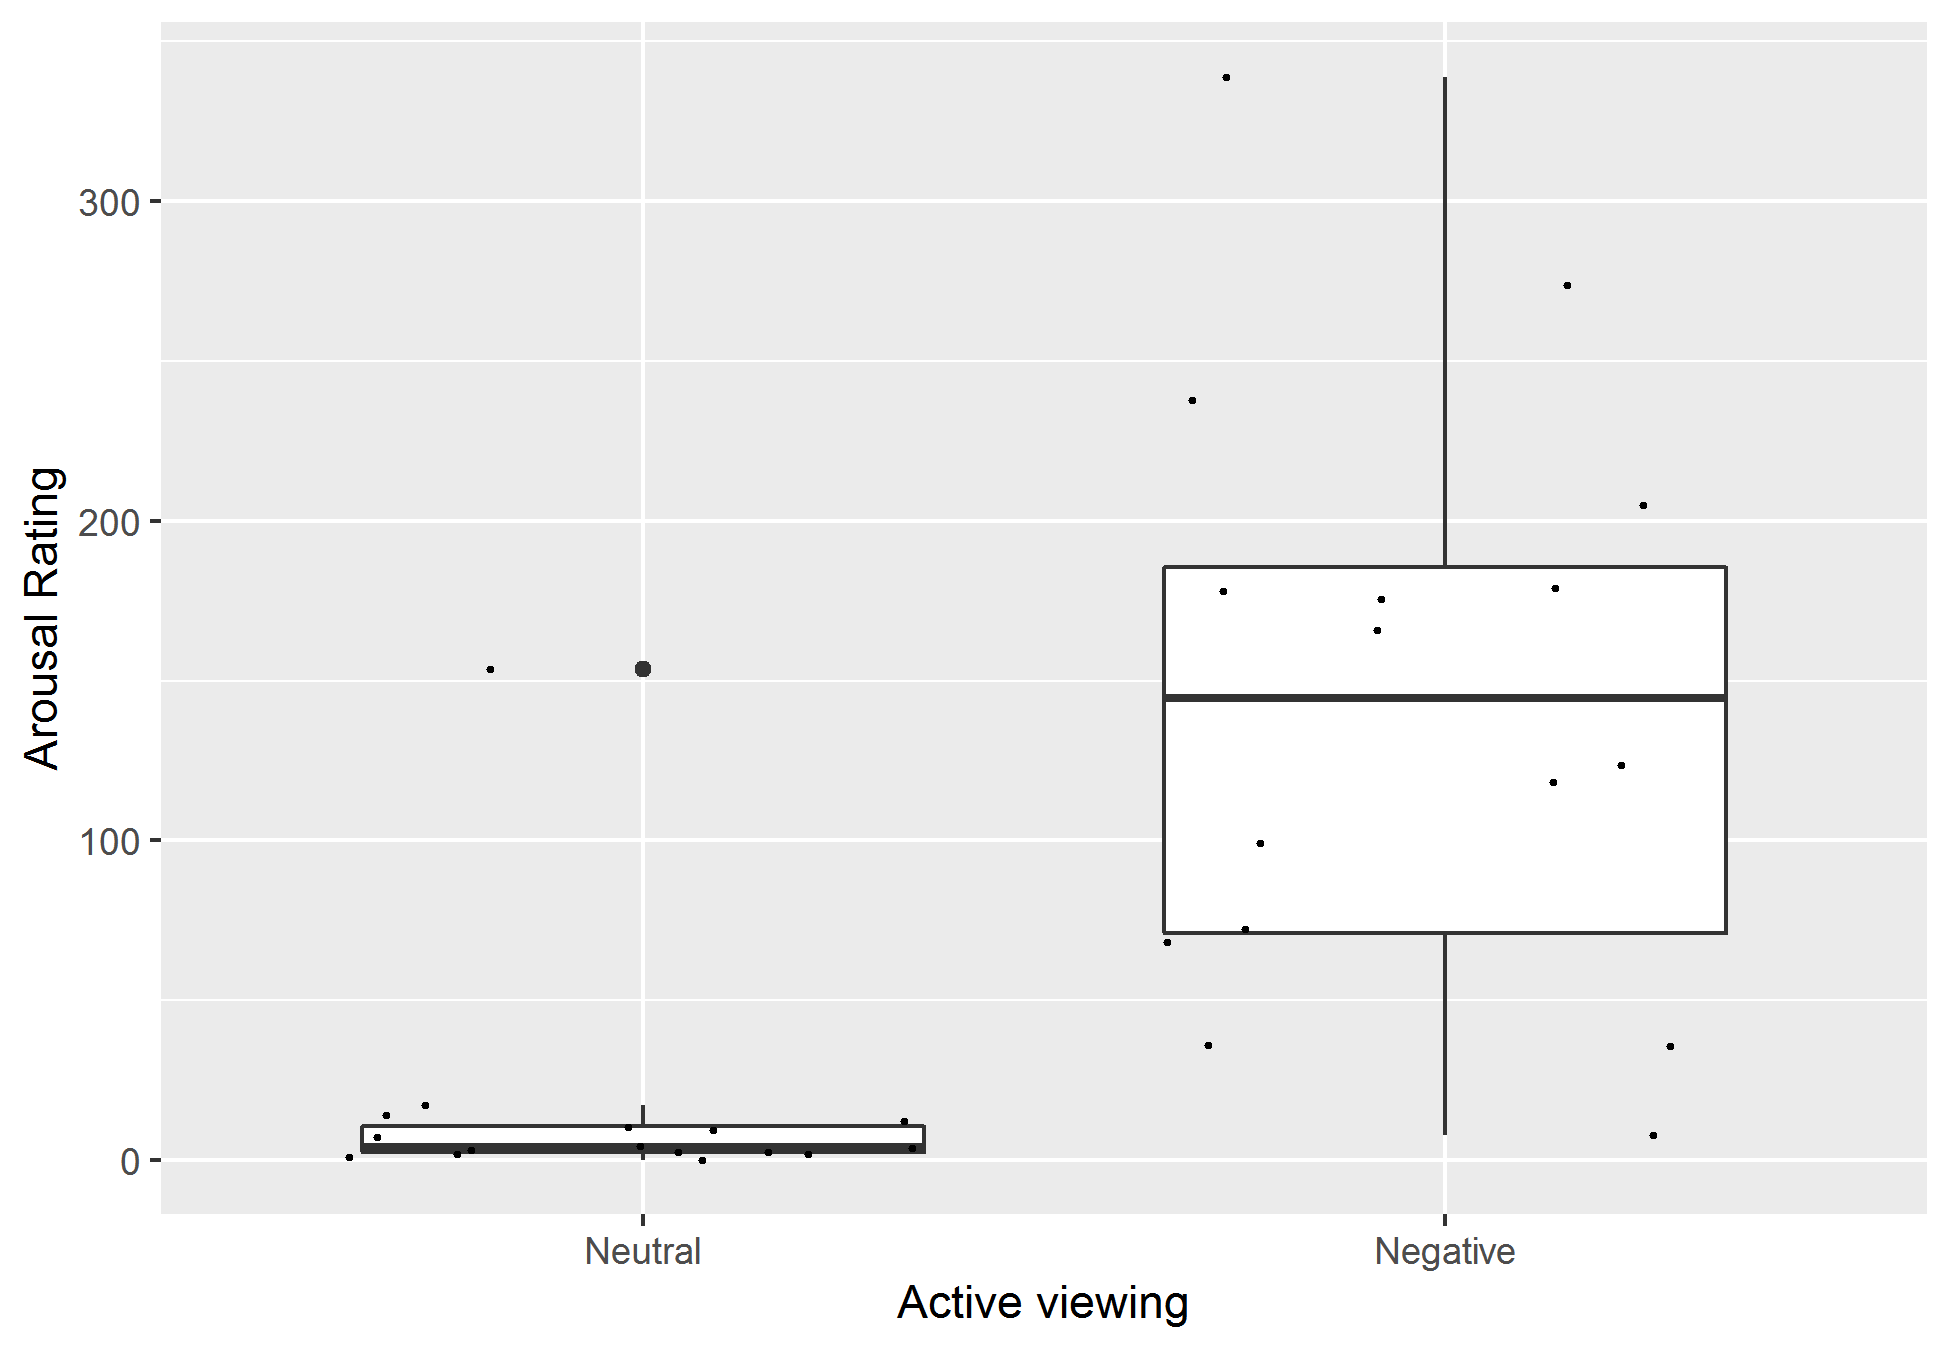
\includegraphics[width=0.75\linewidth]{Manuscript_ERED_Stage1_files/figure-latex/FigSubjArousalViewPilot-1} \caption{Subjective arousal ratings for the conditions "Active viewing - neutral" and "Active viewing - negative" visualized as boxplots. Each dot represents the effort rating of a single subject. Bold dots represent outliers.}\label{fig:FigSubjArousalViewPilot}
\end{figure}

\hypertarget{pilot-study-subjective-arousal-in-the-conditions-active-viewing---negative-distraction-distancing-and-suppression}{%
\subsection{Pilot study: Subjective arousal in the conditions ``Active viewing - negative'', ``Distraction'', ``Distancing'', and ``Suppression''}\label{pilot-study-subjective-arousal-in-the-conditions-active-viewing---negative-distraction-distancing-and-suppression}}

ANOVA:

\begin{tabular}{l|l|l|l|l|l}
\hline
Effect & df & MSE & F & ges & p.value\\
\hline
block & 2.79, 41.89 & 2238.27 & 1.17 & .011 & .332\\
\hline
\end{tabular}

\(BF10=\) 0.11

Paired contrasts:

\begin{table}[H]

\begin{center}
\begin{threeparttable}

\caption{\label{tab:unnamed-chunk-4}Paired contrasts for the rmANOVA comparing subjective arousal of conditions "Active viewing - negative", "Distraction", "Distancing", and "Suppression".}

\begin{tabular}{lllllllll}
\toprule
Contrast & \multicolumn{1}{c}{Estimate} & \multicolumn{1}{c}{$SE$} & \multicolumn{1}{c}{$df$} & \multicolumn{1}{c}{$t$} & \multicolumn{1}{c}{$p$} & \multicolumn{1}{c}{$BF10$} & \multicolumn{1}{c}{$\eta_{p}^{2}$} & \multicolumn{1}{c}{$95\% CI$}\\
\midrule
$View_{negative} - Distraction$ & -0.74 & 16.14 & 45.00 & -0.05 & 1.00 & 0.26 & 4.68e-05 & {}[0.00, 1.00]\\
$View_{negative} - Distancing$ & -5.35 & 16.14 & 45.00 & -0.33 & 1.00 & 0.27 & 2.43e-03 & {}[0.00, 1.00]\\
$View_{negative} - Suppression$ & -26.23 & 16.14 & 45.00 & -1.63 & 0.67 & 1.25 & 0.06 & {}[0.00, 1.00]\\
$Distraction - Distancing$ & -4.61 & 16.14 & 45.00 & -0.29 & 1.00 & 0.26 & 1.81e-03 & {}[0.00, 1.00]\\
$Distraction - Suppression$ & -25.49 & 16.14 & 45.00 & -1.58 & 0.73 & 0.77 & 0.05 & {}[0.00, 1.00]\\
$Distancing - Suppression$ & -20.88 & 16.14 & 45.00 & -1.29 & 1.00 & 0.52 & 0.04 & {}[0.00, 1.00]\\
\bottomrule
\addlinespace
\end{tabular}

\begin{tablenotes}[para]
\normalsize{\textit{Note.} $SE$ = standard error, $df$ = degrees of freedom, $t$ = $t$-statistic, $p$ = $p$-value, CI = confidence interval.}
\end{tablenotes}

\end{threeparttable}
\end{center}

\end{table}

Figure:

\begin{figure}[H]
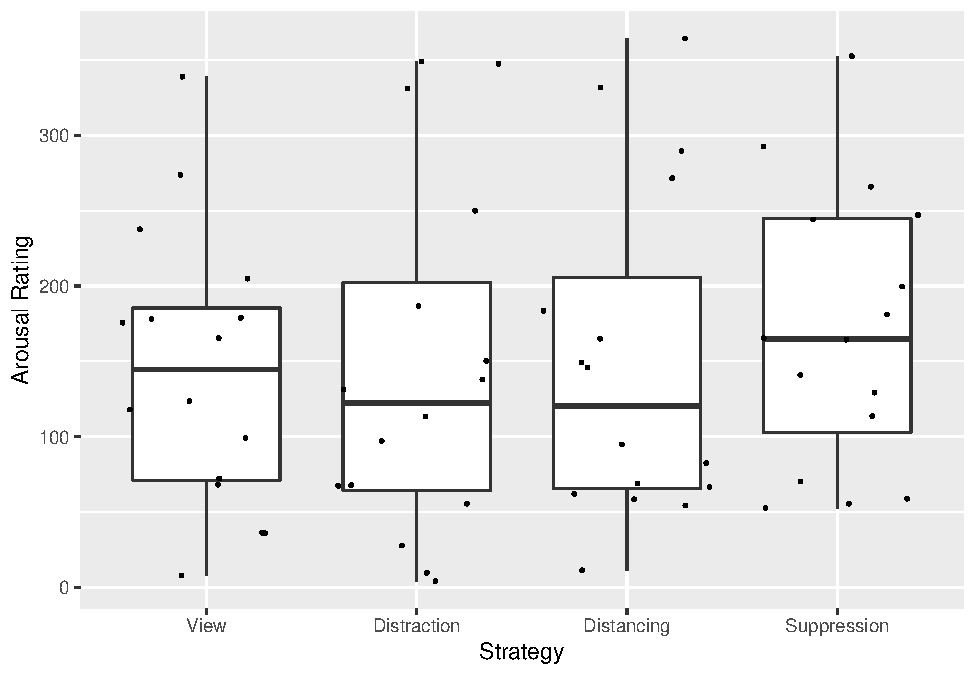
\includegraphics[width=0.75\linewidth]{Manuscript_ERED_Stage1_files/figure-latex/FigSubjArousalRegPilot-1} \caption{Subjective arousal ratings for the conditions "Active viewing - negative", "Distraction", "Distancing", and "Suppression" visualized as boxplots. Each dot represents the effort rating of a single subject. Bold dots represent outliers.}\label{fig:FigSubjArousalRegPilot}
\end{figure}

\hypertarget{pilot-study-physiological-arousal-corrugator-and-levator-activity-in-the-conditions-active-viewing---neutral-and-active-viewing---negative}{%
\subsection{\texorpdfstring{Pilot study: Physiological arousal (\emph{Corrugator} and \emph{Levator} activity) in the conditions ``Active viewing - neutral'' and ``Active viewing - negative''}{Pilot study: Physiological arousal (Corrugator and Levator activity) in the conditions ``Active viewing - neutral'' and ``Active viewing - negative''}}\label{pilot-study-physiological-arousal-corrugator-and-levator-activity-in-the-conditions-active-viewing---neutral-and-active-viewing---negative}}

\emph{Corrugator}:
ANOVA:

\begin{tabular}{l|l|l|l|l|l}
\hline
Effect & df & MSE & F & ges & p.value\\
\hline
block & 1, 15 & 1.01 & 9.70 ** & .237 & .007\\
\hline
\end{tabular}

\(BF10=\) 6,690,401.91

Paired contrasts:

\begin{table}[H]

\begin{center}
\begin{threeparttable}

\caption{\label{tab:unnamed-chunk-5}Paired contrasts for the rmANOVA comparing physiological arousal (*Corrugator* activity) of negative and neutral pictures in the condition "active viewing".}

\begin{tabular}{lllllllll}
\toprule
Contrast & \multicolumn{1}{c}{Estimate} & \multicolumn{1}{c}{$SE$} & \multicolumn{1}{c}{$df$} & \multicolumn{1}{c}{$t$} & \multicolumn{1}{c}{$p$} & \multicolumn{1}{c}{$BF10$} & \multicolumn{1}{c}{$\eta_{p}^{2}$} & \multicolumn{1}{c}{$95\% CI$}\\
\midrule
$View_{neutral} - View_{negative}$ & -1.11 & 0.36 & 15.00 & -3.11 & 0.01 & 5,019,313.20 & 0.39 & {}[0.09, 1.00]\\
\bottomrule
\addlinespace
\end{tabular}

\begin{tablenotes}[para]
\normalsize{\textit{Note.} $SE$ = standard error, $df$ = degrees of freedom, $t$ = $t$-statistic, $p$ = $p$-value, CI = confidence interval.}
\end{tablenotes}

\end{threeparttable}
\end{center}

\end{table}

\emph{Levator}:
ANOVA:

\begin{tabular}{l|l|l|l|l|l}
\hline
Effect & df & MSE & F & ges & p.value\\
\hline
block & 1, 15 & 0.17 & 7.72 * & .162 & .014\\
\hline
\end{tabular}

\(BF10=\) 48.44

Paired contrasts:

\begin{table}[H]

\begin{center}
\begin{threeparttable}

\caption{\label{tab:unnamed-chunk-6}Paired contrasts for the rmANOVA comparing physiological arousal (*Levator* activity) of negative and neutral pictures in the condition "active viewing".}

\begin{tabular}{lllllllll}
\toprule
Contrast & \multicolumn{1}{c}{Estimate} & \multicolumn{1}{c}{$SE$} & \multicolumn{1}{c}{$df$} & \multicolumn{1}{c}{$t$} & \multicolumn{1}{c}{$p$} & \multicolumn{1}{c}{$BF10$} & \multicolumn{1}{c}{$\eta_{p}^{2}$} & \multicolumn{1}{c}{$95\% CI$}\\
\midrule
$View_{neutral} - View_{negative}$ & -0.40 & 0.14 & 15.00 & -2.78 & 0.01 & 41.02 & 0.34 & {}[0.05, 1.00]\\
\bottomrule
\addlinespace
\end{tabular}

\begin{tablenotes}[para]
\normalsize{\textit{Note.} $SE$ = standard error, $df$ = degrees of freedom, $t$ = $t$-statistic, $p$ = $p$-value, CI = confidence interval.}
\end{tablenotes}

\end{threeparttable}
\end{center}

\end{table}

Figures:

\begin{figure}[H]
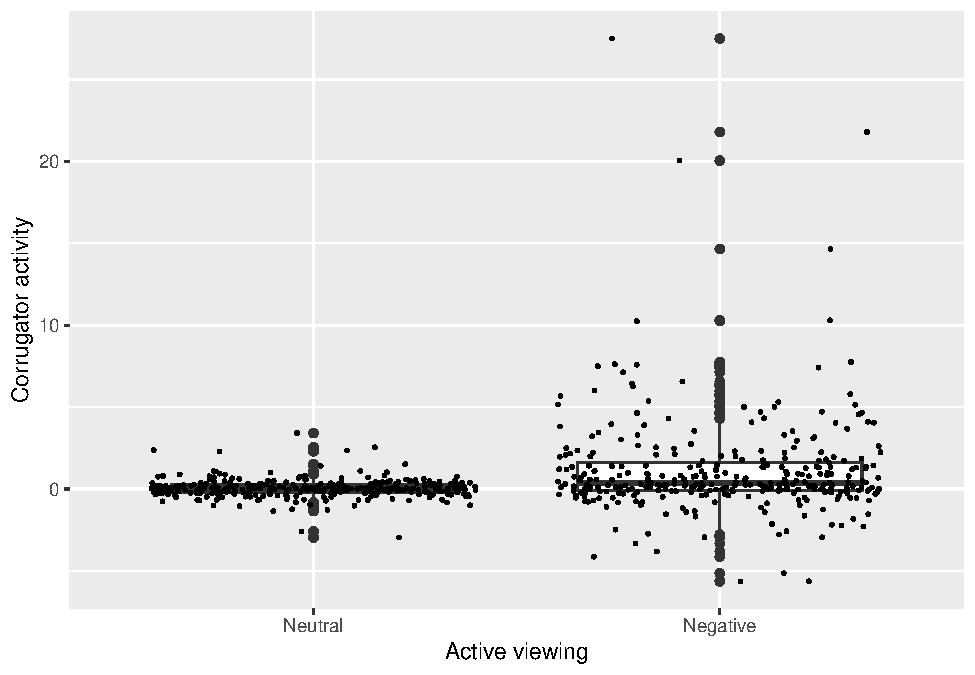
\includegraphics[width=0.75\linewidth]{Manuscript_ERED_Stage1_files/figure-latex/FigEMGCorrViewPilot-1} \caption{Corrugator activity for the conditions "Active viewing - neutral" and "Active viewing - negative" visualized as boxplots. Each dot represents the corrugator activity of a single trial. Bold dots represent outliers.}\label{fig:FigEMGCorrViewPilot}
\end{figure}
\begin{figure}[H]
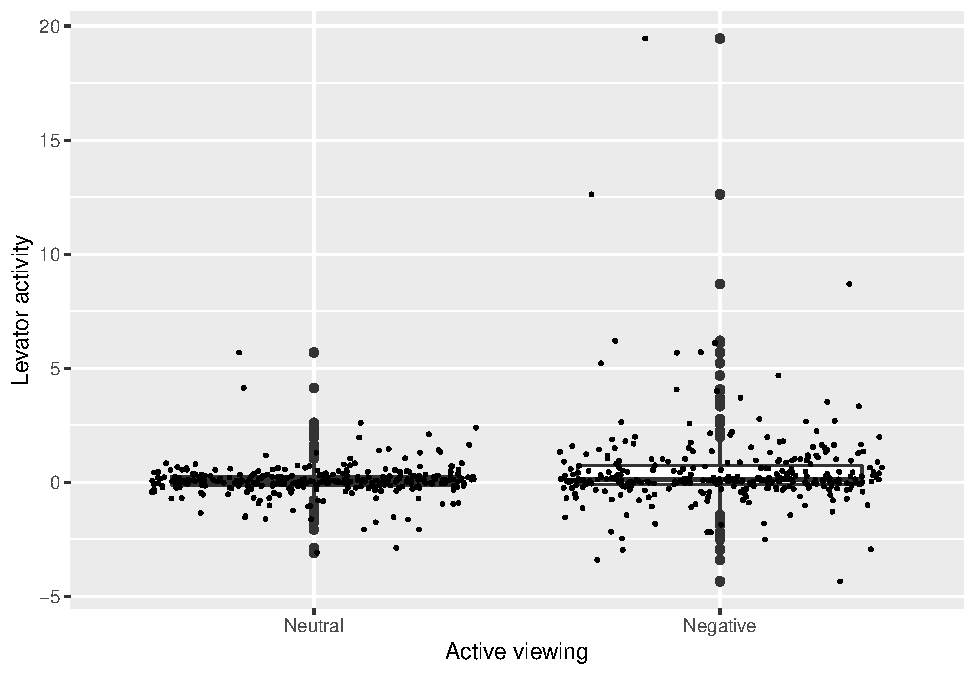
\includegraphics[width=0.75\linewidth]{Manuscript_ERED_Stage1_files/figure-latex/FigEMGLevViewPilot-1} \caption{Levator activity for the conditions "Active viewing - neutral" and "Active viewing - negative" visualized as boxplots. Each dot represents the levator activity of a single trial. Bold dots represent outliers.}\label{fig:FigEMGLevViewPilot}
\end{figure}

\hypertarget{pilot-study-physiological-arousal-corrugator-and-levator-activity-in-the-conditionsactive-viewing---negative-distraction-distancing-and-suppression}{%
\subsection{\texorpdfstring{Pilot study: Physiological arousal (\emph{Corrugator} and \emph{Levator} activity) in the conditions``Active viewing - negative'', ``Distraction'', ``Distancing'', and ``Suppression''}{Pilot study: Physiological arousal (Corrugator and Levator activity) in the conditions``Active viewing - negative'', ``Distraction'', ``Distancing'', and ``Suppression''}}\label{pilot-study-physiological-arousal-corrugator-and-levator-activity-in-the-conditionsactive-viewing---negative-distraction-distancing-and-suppression}}

\emph{Corrugator}:
ANOVA:

\begin{tabular}{l|l|l|l|l|l}
\hline
Effect & df & MSE & F & ges & p.value\\
\hline
block & 1.53, 22.98 & 1.16 & 5.71 * & .189 & .015\\
\hline
\end{tabular}

\(BF10=\) 5,257,689.54

Paired contrasts:

\begin{table}[H]

\begin{center}
\begin{threeparttable}

\caption{\label{tab:unnamed-chunk-7}Paired contrasts for the rmANOVA comparing physiological arousal (*Corrugator* activity) of conditions "Active viewing - negative", "Distraction", "Distancing", and "Suppression".}

\begin{tabular}{lllllllll}
\toprule
Contrast & \multicolumn{1}{c}{Estimate} & \multicolumn{1}{c}{$SE$} & \multicolumn{1}{c}{$df$} & \multicolumn{1}{c}{$t$} & \multicolumn{1}{c}{$p$} & \multicolumn{1}{c}{$BF10$} & \multicolumn{1}{c}{$\eta_{p}^{2}$} & \multicolumn{1}{c}{$95\% CI$}\\
\midrule
$View_{negative} - Distraction$ & 0.88 & 0.27 & 45.00 & 3.22 & 0.01 & 4,962.89 & 0.19 & {}[0.05, 1.00]\\
$View_{negative} - Distancing$ & 0.95 & 0.27 & 45.00 & 3.50 & 0.01 & 616.63 & 0.21 & {}[0.06, 1.00]\\
$View_{negative} - Suppression$ & 0.92 & 0.27 & 45.00 & 3.40 & 0.01 & 11,678.82 & 0.20 & {}[0.06, 1.00]\\
$Distraction - Distancing$ & 0.08 & 0.27 & 45.00 & 0.28 & 1.00 & 0.07 & 1.78e-03 & {}[0.00, 1.00]\\
$Distraction - Suppression$ & 0.05 & 0.27 & 45.00 & 0.18 & 1.00 & 0.08 & 7.22e-04 & {}[0.00, 1.00]\\
$Distancing - Suppression$ & -0.03 & 0.27 & 45.00 & -0.10 & 1.00 & 0.06 & 2.36e-04 & {}[0.00, 1.00]\\
\bottomrule
\addlinespace
\end{tabular}

\begin{tablenotes}[para]
\normalsize{\textit{Note.} $SE$ = standard error, $df$ = degrees of freedom, $t$ = $t$-statistic, $p$ = $p$-value, CI = confidence interval.}
\end{tablenotes}

\end{threeparttable}
\end{center}

\end{table}

\emph{Levator}:
ANOVA:

\begin{tabular}{l|l|l|l|l|l}
\hline
Effect & df & MSE & F & ges & p.value\\
\hline
block & 2.07, 31.00 & 0.20 & 8.27 ** & .225 & .001\\
\hline
\end{tabular}

\(BF10=\) 672,341.29

Paired contrasts:

\begin{table}[H]

\begin{center}
\begin{threeparttable}

\caption{\label{tab:unnamed-chunk-8}Paired contrasts for the rmANOVA comparing physiological arousal (*Levator* activity) of conditions "Active viewing - negative", "Distraction", "Distancing", and "Suppression".}

\begin{tabular}{lllllllll}
\toprule
Contrast & \multicolumn{1}{c}{Estimate} & \multicolumn{1}{c}{$SE$} & \multicolumn{1}{c}{$df$} & \multicolumn{1}{c}{$t$} & \multicolumn{1}{c}{$p$} & \multicolumn{1}{c}{$BF10$} & \multicolumn{1}{c}{$\eta_{p}^{2}$} & \multicolumn{1}{c}{$95\% CI$}\\
\midrule
$View_{negative} - Distraction$ & 0.42 & 0.13 & 45.00 & 3.24 & 0.01 & 58.02 & 0.19 & {}[0.05, 1.00]\\
$View_{negative} - Distancing$ & 0.45 & 0.13 & 45.00 & 3.46 & 0.01 & 93.49 & 0.21 & {}[0.06, 1.00]\\
$View_{negative} - Suppression$ & 0.62 & 0.13 & 45.00 & 4.79 & 0.00 & 6,253.91 & 0.34 & {}[0.16, 1.00]\\
$Distraction - Distancing$ & 0.03 & 0.13 & 45.00 & 0.22 & 1.00 & 0.07 & 1.06e-03 & {}[0.00, 1.00]\\
$Distraction - Suppression$ & 0.20 & 0.13 & 45.00 & 1.54 & 0.78 & 1.52 & 0.05 & {}[0.00, 1.00]\\
$Distancing - Suppression$ & 0.17 & 0.13 & 45.00 & 1.32 & 1.00 & 0.52 & 0.04 & {}[0.00, 1.00]\\
\bottomrule
\addlinespace
\end{tabular}

\begin{tablenotes}[para]
\normalsize{\textit{Note.} $SE$ = standard error, $df$ = degrees of freedom, $t$ = $t$-statistic, $p$ = $p$-value, CI = confidence interval.}
\end{tablenotes}

\end{threeparttable}
\end{center}

\end{table}

Figures:

\begin{figure}[H]
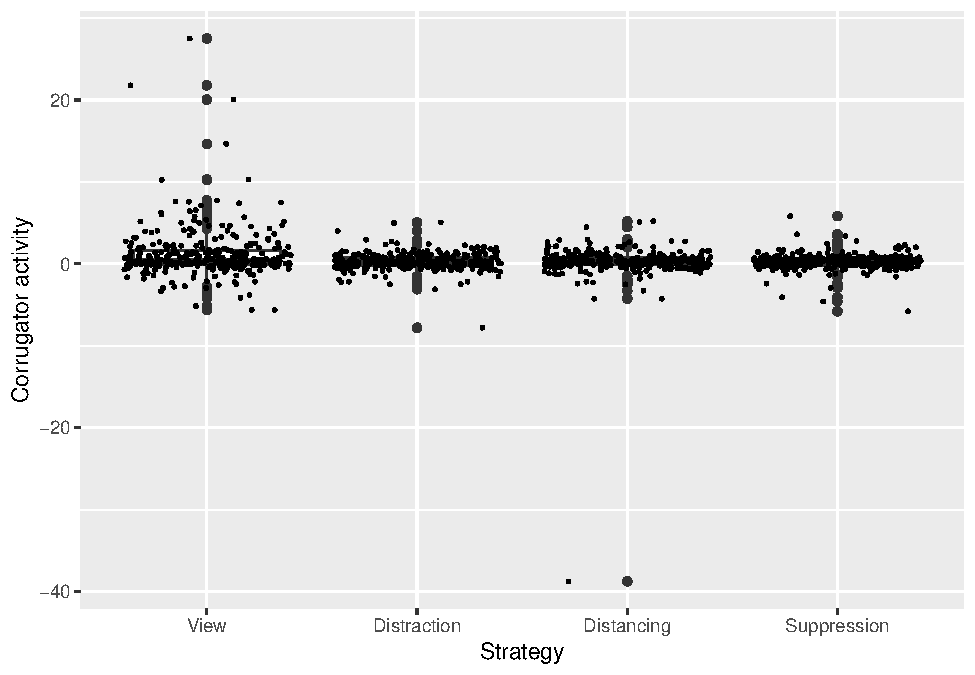
\includegraphics[width=0.75\linewidth]{Manuscript_ERED_Stage1_files/figure-latex/FigEMGCorrRegPilot-1} \caption{Corrugator activity for the conditions "Active viewing - negative", "Distraction", "Distancing", and "Suppression" visualized as boxplots. Each dot represents the corrugator activity of a single trial. Bold dots represent outliers.}\label{fig:FigEMGCorrRegPilot}
\end{figure}
\begin{figure}[H]
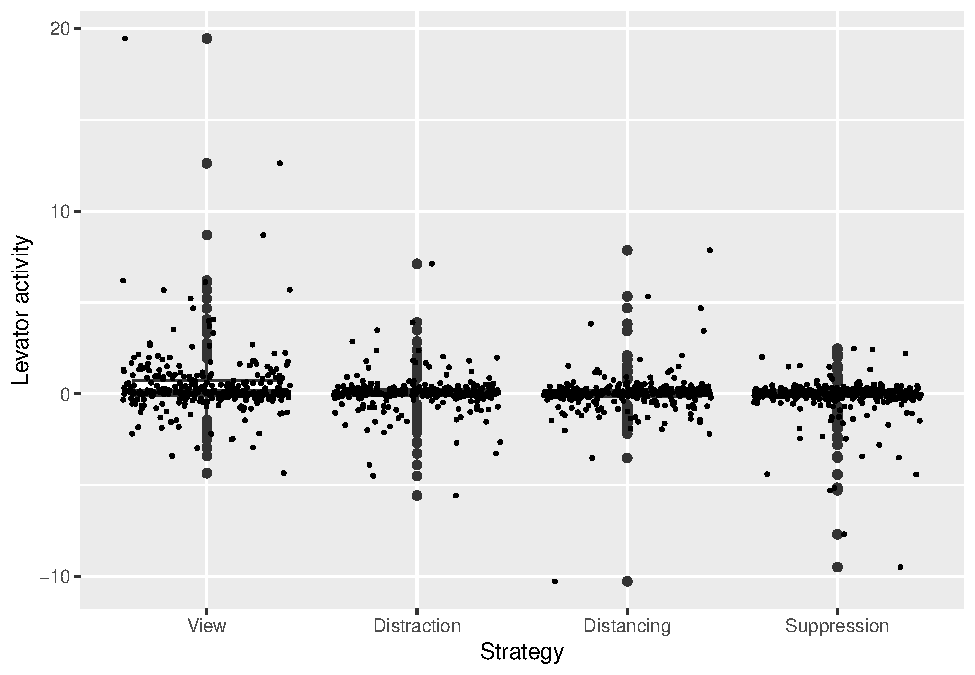
\includegraphics[width=0.75\linewidth]{Manuscript_ERED_Stage1_files/figure-latex/FigEMGLevRegPilot-1} \caption{Levator activity for the conditions "Active viewing - negative", "Distraction", "Distancing", and "Suppression" visualized as boxplots. Each dot represents the levator activity of a single trial. Bold dots represent outliers.}\label{fig:FigEMGLevRegPilot}
\end{figure}

\hypertarget{pilot-study-subjective-effort-in-the-conditions-active-viewing---negative-distraction-distancing-and-suppression}{%
\subsection{Pilot study: Subjective effort in the conditions ``Active viewing - negative'', ``Distraction'', ``Distancing'', and ``Suppression''}\label{pilot-study-subjective-effort-in-the-conditions-active-viewing---negative-distraction-distancing-and-suppression}}

ANOVA:

\begin{tabular}{l|l|l|l|l|l}
\hline
Effect & df & MSE & F & ges & p.value\\
\hline
block & 2.38, 35.66 & 4388.19 & 11.13 *** & .185 & <.001\\
\hline
\end{tabular}

\(BF10=\) 7.40

Paired contrasts:

\begin{table}[H]

\begin{center}
\begin{threeparttable}

\caption{\label{tab:unnamed-chunk-9}Paired contrasts for the rmANOVA comparing subjective effort of conditions "Active viewing - negative", "Distraction", "Distancing", and "Suppression".}

\begin{tabular}{lllllllll}
\toprule
Contrast & \multicolumn{1}{c}{Estimate} & \multicolumn{1}{c}{$SE$} & \multicolumn{1}{c}{$df$} & \multicolumn{1}{c}{$t$} & \multicolumn{1}{c}{$p$} & \multicolumn{1}{c}{$BF10$} & \multicolumn{1}{c}{$\eta_{p}^{2}$} & \multicolumn{1}{c}{$95\% CI$}\\
\midrule
$View_{negative} - Distancing$ & -110.72 & 20.85 & 45.00 & -5.31 & 0.00 & 59.77 & 0.39 & {}[0.20, 1.00]\\
$View_{negative} - Distraction$ & -89.72 & 20.85 & 45.00 & -4.30 & 0.00 & 20.49 & 0.29 & {}[0.12, 1.00]\\
$View_{negative} - Suppression$ & -88.15 & 20.85 & 45.00 & -4.23 & 0.00 & 33.13 & 0.28 & {}[0.11, 1.00]\\
$Distraction - Distancing$ & 21.00 & 20.85 & 45.00 & 1.01 & 1.00 & 0.50 & 0.02 & {}[0.00, 1.00]\\
$Distraction - Suppression$ & 22.57 & 20.85 & 45.00 & 1.08 & 1.00 & 0.57 & 0.03 & {}[0.00, 1.00]\\
$Distancing - Suppression$ & 1.57 & 20.85 & 45.00 & 0.08 & 1.00 & 0.26 & 1.27e-04 & {}[0.00, 1.00]\\
\bottomrule
\addlinespace
\end{tabular}

\begin{tablenotes}[para]
\normalsize{\textit{Note.} $SE$ = standard error, $df$ = degrees of freedom, $t$ = $t$-statistic, $p$ = $p$-value, CI = confidence interval.}
\end{tablenotes}

\end{threeparttable}
\end{center}

\end{table}

Figure:

\begin{figure}[H]
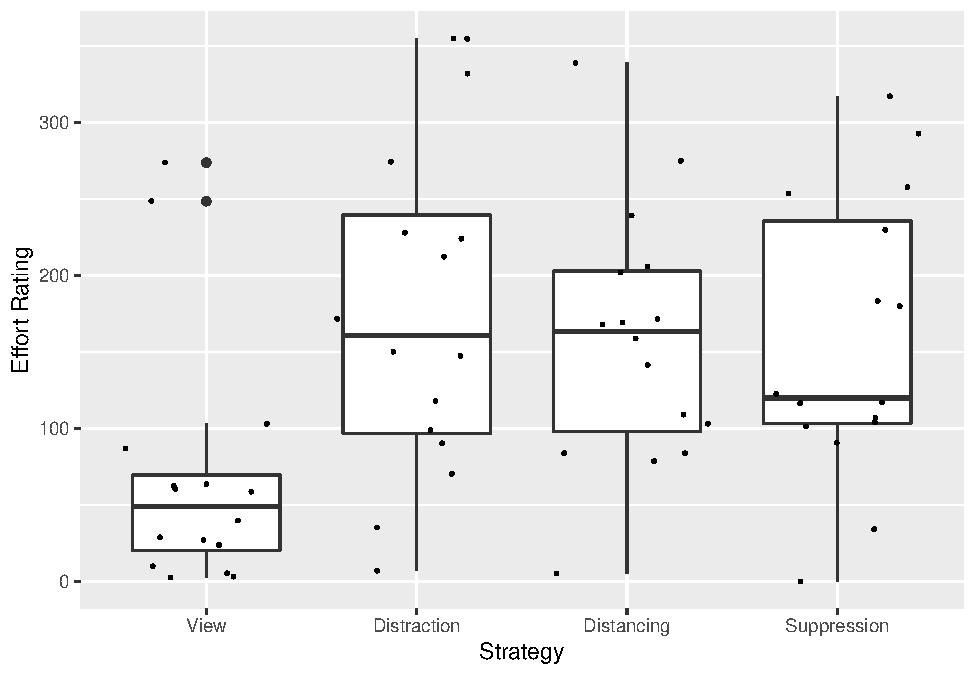
\includegraphics[width=0.75\linewidth]{Manuscript_ERED_Stage1_files/figure-latex/FigSubjEffortPilot-1} \caption{Subjective effort ratings for the conditions "Active viewing - negative", "Distraction", "Distancing", and "Suppression" visualized as boxplots. Each dot represents the effort rating of a single subject. Bold dots represent outliers.}\label{fig:FigSubjEffortPilot}
\end{figure}


\end{document}
